\documentclass[11pt,letterpaper]{article}

% --- Typography & Layout ---
\usepackage[margin=1in]{geometry}
\usepackage{setspace}
\onehalfspacing
\usepackage[T1]{fontenc}
\usepackage[utf8]{inputenc}
\usepackage{microtype}
\usepackage{lmodern}

% --- Math Packages ---
\usepackage{amsmath,amssymb,amsfonts,bm}
\usepackage{mathtools}

% --- Tables & Figures ---
\usepackage{booktabs}
\usepackage{tabularx}
\usepackage{array}
\usepackage{makecell}
\usepackage{graphicx}
\usepackage[font=small,labelfont=bf,tableposition=top]{caption}
\usepackage{subcaption}

% --- Colors & Links ---
\usepackage[dvipsnames]{xcolor}
\usepackage[colorlinks=true,linkcolor=MidnightBlue,citecolor=MidnightBlue,urlcolor=MidnightBlue]{hyperref}

% --- Bibliography ---
\usepackage[round]{natbib}

% --- Custom Math Notation ---
\newcommand{\JSD}{\operatorname{JSD}}
\newcommand{\dself}{d_{\mathrm{self}}}
\newcommand{\dref}{d_{\mathrm{ref}}}
\newcommand{\Turnover}{\mathrm{Turnover}}
\newcommand{\Jaccard}{\mathrm{Jaccard}}

\title{\textbf{\Large The Persistent Architecture of Relational Investment:\\Social Signatures in the NetHealth Study}}

\author{\textbf{Omar Lizardo}\\[0.5em]
\textit{Department of Sociology, University of California, Los Angeles}\\
\textit{NetHealth Research Collaboration}}

\date{\today}

\begin{document}

\maketitle

\begin{abstract}
\noindent How do individuals allocate cognitive, temporal, and emotional bandwidth across their personal networks? Using high-resolution digital call records paired with eight waves of longitudinal network and psychometric surveys from the NetHealth study ($N = 491$ egos, 498,237 communication events), this paper investigates the structure, temporal stability, and psychological foundations of \textbf{social signatures}---the ranked proportion of communication effort allocated across alters within discrete temporal windows. We demonstrate that the core signature persistence hypothesis holds across multiple timescales (academic years, semesters, quarters, months, and rolling weekly windows): intra-individual self-divergence ($\dself$) is uniformly and overwhelmingly smaller than inter-individual reference divergence ($\dref$, $p < 10^{-12}$ across all resolutions). Parametric evaluations confirm that power-law models ($p(r) \sim r^{-\alpha}$, mean $R^2 = 0.935$) fit empirical signatures significantly better than exponential decay models, with ego-specific decay exponents ($\alpha$) converging to an asymptotic value within 6 to 8 months of continuous observation. Going beyond previous work, we introduce three substantive theoretical expansions: (1) \textbf{Functional Support Grounding}: Linking communication ranks to multi-dimensional survey nominations ($N = 13,174$ dyads), we reveal that the steep drop in communication effort corresponds to sharp qualitative transitions from family-dominated instrumental and emotional support (Rank 1: 69.7\% kin, 85.4\% emotional support, 87.6\% advice) to friend-dominated companionship at lower ranks; (2) \textbf{The Slot-Filling Dynamic}: We show that high signature stability persists despite massive alter turnover (averaging 80.1\% across semesters), providing direct evidence that college students replenish relational slots with new alters rather than restructuring their overall allocation profile; and (3) \textbf{Psychological Determinants}: Using longitudinal mixed-effects and cross-sectional models, we demonstrate that Neuroticism strongly predicts steeper, hyper-concentrated signatures ($\beta = 0.098, p < 10^{-6}$), revealing that emotional vulnerability drives disproportionate reliance on core ties.
\end{abstract}

\vspace{1em}
\noindent\textbf{Keywords:} Social Signatures, Egocentric Networks, NetHealth, Jensen-Shannon Divergence, Tie Strength, Slot-Filling Hypothesis, Personality Traits.

\newpage

\section{Introduction and Theoretical Background}

A central premise in evolutionary anthropology and structural sociology is that human sociality is governed by cognitive and temporal limits on relational investment \citep{dunbar1992neocortex,dunbar1998social,miritello2013time}. While an individual may recognize hundreds of acquaintances, active personal networks are structured into concentric, hierarchical layers: an intimate core of 1 to 2 primary confidants, a sympathy group of approximately 5 close ties, an affinity group of 12 to 15 active alters, and expanding outer circles of declining emotional intensity and contact frequency \citep{dunbar2018anatomy,roberts2009exploring,sutcliffe2012relationships}.

In a foundational contribution, \citet{saramaeki2014persistence} operationalized this relational hierarchy as an individual's \textbf{social signature}: the relative distribution of communication effort that an individual (ego) directs toward their alters, ordered from most-frequently to least-frequently contacted within a given window of observation. Tracking high school graduates transitioning into university using mobile call detail records, Saram{\"a}ki and colleagues established two defining regularities: first, social signatures vary substantially across individuals; and second, an individual's social signature exhibits remarkable intra-individual persistence over time, remaining stable even when the specific alters occupying the network turn over substantially. Subsequent investigations demonstrated that persistent signature patterns generalize across multiple communication channels, including voice calls and text messaging \citep{heydari2018multichannel,kikas2013burstiness}.

Despite these important empirical breakthroughs, significant theoretical and empirical gaps remain in our understanding of personal communication architectures. First, existing studies have relied primarily on call logs from commercial telecommunications providers. Because commercial telecommunications data lack relational content, researchers have been unable to determine whether the steep mathematical drop-off in communication frequency corresponds to qualitative differences in social support---such as emotional comfort, instrumental advice, companionship, or financial assistance. Second, the behavioral mechanisms underlying signature persistence remain ambiguous: does an individual's signature remain stable because their core ties are immutable, or do individuals actively preserve their structural signature by ``slotting'' newly acquired alters into vacant relational positions? Third, prior research has largely neglected the psychological dispositions and well-being correlates that give rise to distinct signature shapes \citep{centellegher2017personality}. Why do some individuals maintain steep, hyper-concentrated communication profiles focused on a single alter, while others sustain broad, egalitarian distributions of attention?

This paper addresses these foundational questions by drawing on the \textbf{NetHealth Project}---a comprehensive, multi-year cohort study tracking undergraduate students at the University of Notre Dame. By integrating two full years of continuous, passive smartphone communication logs (498,237 outgoing voice call records) with dense 8-wave sociocentric network surveys, alter-alter structural edge lists, and longitudinal psychometric batteries, we examine the persistence, mathematical form, functional grounding, and psychological origins of social signatures during a major life-course transition.

\section{Data and Methodology}

\subsection{The NetHealth Dataset}
The NetHealth study recruited an entire incoming cohort of first-year undergraduate students at the University of Notre Dame beginning in Fall 2015. Participants consented to continuous digital sensing via their smartphones and Fitbit devices, alongside dense sociocentric network and psychological surveys administered at regular intervals across their college careers. 

Our analytical design links five primary data streams:
\begin{enumerate}
    \item \textbf{Continuous Communication Logs}: 498,237 outgoing voice call events collected from participant iOS devices spanning June 30, 2015 through July 2, 2017 across 491 unique egos.
    \item \textbf{Academic Calendar}: Comprehensive institutional records documenting semester start and end dates, examination periods, orientation, and vacation breaks.
    \item \textbf{Sociocentric Network Surveys}: 35,913 alter nominations gathered across 8 longitudinal survey waves recording tie categories (family kin vs.\ peer friends), perceived closeness, interpersonal trust, and multidimensional social support.
    \item \textbf{Alter-Alter Edge Lists}: 174,748 structural ties connecting peers within each respondent's personal egocentric network across survey waves.
    \item \textbf{Basic Psychometric Batteries}: Longitudinal survey instruments measuring the Big Five personality dimensions (Extraversion, Agreeableness, Conscientiousness, Neuroticism, Openness), the CES-D Depression Scale, and the UCLA Loneliness Scale.
\end{enumerate}

\subsection{Temporal Window Binning and Filtering}
To establish whether social signatures persist across differing temporal resolutions, we construct two complementary binning architectures:
\begin{itemize}
    \item \textbf{Calendar-Based Windows} (July 1, 2015 -- June 30, 2017):
    \begin{itemize}
        \item \textit{Academic Years} ($W = 2$): July 2015 -- June 2016; July 2016 -- June 2017.
        \item \textit{Semesters} ($W = 4$): Fall 2015, Spring 2016, Fall 2016, Spring 2017.
        \item \textit{Quarters} ($W = 8$): July--September, October--December, January--March, April--June.
        \item \textit{Months} ($W = 24$): 24 consecutive calendar months.
    \end{itemize}
    \item \textbf{Week-Based Windows} (July 6, 2015 -- July 2, 2017; 104 Monday--Sunday weeks):
    \begin{itemize}
        \item \textit{3-Week Rolling Windows} ($W = 102$): 3-week moving windows in 1-week increments.
        \item \textit{2-Week Discrete Windows} ($W = 52$): Non-overlapping 14-day intervals.
        \item \textit{1-Week Discrete Windows} ($W = 104$): 7-day intervals.
    \end{itemize}
\end{itemize}

To ensure that estimated signatures reflect meaningful personal communication structures, egos are required to meet two standard inclusion criteria: (a) a minimum of 2 active alters in every window ($k_{i,w} \ge 2$), and (b) an average call volume exceeding 10 calls per window. When comparing across calendar definitions, we evaluate the common intersection cohort ($N = 147$ egos).

\begin{table}[htbp]
\centering
\caption{NetHealth Cohort Summary Across Temporal Window Definitions}
\label{tab:cohort_summary}
\small
\resizebox{\textwidth}{!}{%
\begin{tabular}{lcccc}
\toprule
\textbf{Window Scheme} & \textbf{Window Span} & \textbf{Windows ($W$)} & \textbf{Eligibility Criteria} & \textbf{Eligible Egos ($N$)} \\
\midrule
Academic Years & Jul 2015 -- Jun 2017 & 2 & $\ge 2$ alters, $>10$ calls & 388 \\
Semesters & Jul 2015 -- Jun 2017 & 4 & $\ge 2$ alters, $>10$ calls & 290 \\
Quarters & Jul 2015 -- Jun 2017 & 8 & $\ge 2$ alters, $>10$ calls & 227 \\
Months & Jul 2015 -- Jun 2017 & 24 & $\ge 2$ alters, $>10$ calls & 147 \\
Common Calendar Cohort & Jul 2015 -- Jun 2017 & -- & All 4 calendar schemes & 147 \\
3-Week Rolling & Jul 2015 -- Jul 2017 & 102 & $\ge 2$ alters, $>10$ calls & 88 \\
2-Week Discrete & Jul 2015 -- Jul 2017 & 52 & $\ge 2$ alters, $>10$ calls & 65 \\
1-Week Discrete & Jul 2015 -- Jul 2017 & 104 & $\ge 2$ alters, $>10$ calls & 14 \\
\bottomrule
\end{tabular}%
}
\end{table}

\subsection{Mathematical Formulation of Social Signatures and Jensen-Shannon Divergence}
For ego $i$ in temporal window $w$, communication weights $w_{i,j,w}$ (measured as total outgoing voice calls) to alters $j = 1, \dots, k_{i,w}$ are sorted in descending order:
\begin{equation}
w_{i,(1),w} \ge w_{i,(2),w} \ge \dots \ge w_{i,(k),w}
\end{equation}
The social signature is defined as the normalized vector of interaction proportions:
\begin{equation}
p_{i,w}(r) = \frac{w_{i,(r),w}}{W_{i,w}}, \quad \text{where } W_{i,w} = \sum_{j=1}^{k_{i,w}} w_{i,j,w} \quad \text{and} \quad \sum_{r=1}^{k_{i,w}} p_{i,w}(r) = 1
\end{equation}
where $r \in \{1, 2, \dots, k_{i,w}\}$ represents the alter rank.

To quantify the similarity or difference between two probability vectors $P = \{p_r\}_{r=1}^{k_1}$ and $Q = \{q_r\}_{r=1}^{k_2}$ of potentially unequal lengths $k_1 \neq k_2$, we append zeros to the shorter distribution up to length $K = \max(k_1, k_2)$ on-the-fly and compute the \textbf{Jensen-Shannon Divergence} \citep[JSD;][]{lin1991divergence}:
\begin{equation}
\JSD(P \parallel Q) = H(M) - \frac{1}{2}\left[H(P) + H(Q)\right]
\end{equation}
where $M = \frac{1}{2}(P + Q)$ is the mixture distribution, and $H(P)$ denotes Shannon entropy measured in bits:
\begin{equation}
H(P) = -\sum_{r=1}^{K} p_r \log_2(p_r) \quad (\text{with } 0 \log_2 0 \equiv 0)
\end{equation}
JSD is symmetric ($\JSD(P \parallel Q) = \JSD(Q \parallel P)$), non-negative, and strictly bounded between 0 (identical distributions) and 1 bit (disjoint distributions).

For evaluating consistency across multiple observation windows simultaneously, we also compute the generalized $n$-ary Jensen-Shannon divergence across a set of $n$ distributions $\{P_1, P_2, \dots, P_n\}$:
\begin{equation}
\JSD(P_1, \dots, P_n) = H\left(\frac{1}{n}\sum_{m=1}^n P_m\right) - \frac{1}{n}\sum_{m=1}^n H(P_m)
\end{equation}

We define two core divergence metrics:
\begin{enumerate}
    \item \textbf{Self-Divergence ($\dself$)}: The mean pairwise JSD between consecutive temporal windows for the same ego across observation periods:
    \begin{equation}
    \dself(i) = \frac{1}{W-1} \sum_{w=1}^{W-1} \JSD(P_{i,w} \parallel P_{i,w+1})
    \end{equation}
    \item \textbf{Reference-Divergence ($\dref$)}: The divergence between the social signatures of distinct individuals observed within the same temporal window:
    \begin{align}
    \text{By Ego: } \dref(i) &= \frac{1}{W} \sum_{w=1}^W \left[ \frac{1}{n_w - 1} \sum_{j \neq i} \JSD(P_{i,w} \parallel P_{j,w}) \right] \\
    \text{All Pairs: } \bar{d}_{\mathrm{ref}} &= \frac{1}{\binom{n}{2}} \sum_{i < j} \left[ \frac{1}{W} \sum_{w=1}^W \JSD(P_{i,w} \parallel P_{j,w}) \right]
    \end{align}
\end{enumerate}

If personal social signatures exhibit persistent idiosyncratic stability over time, an individual's self-divergence must be systematically and significantly smaller than the reference divergence observed between random peers ($\dself < \dref$).

\section{Empirical Results: Persistence and Parametric Architecture}

\subsection{Empirical Social Signatures}
Figure~\ref{fig:mean_signatures} displays empirical social signatures averaged across egos for ranks 1 through 15 across temporal window definitions. Across all timescales, communication effort exhibits pronounced skewness:
\begin{itemize}
    \item The single top-ranked alter ($r = 1$) commands \textbf{35\% to 45\%} of an ego's total communication bandwidth.
    \item The second-ranked alter ($r = 2$) captures \textbf{18\% to 22\%}.
    \item The top 3 alters collectively account for over \textbf{70\%} of total outgoing interaction volume.
    \item Beyond rank 5, communication drops below 4\% per alter.
\end{itemize}

\begin{figure}[htbp]
\centering
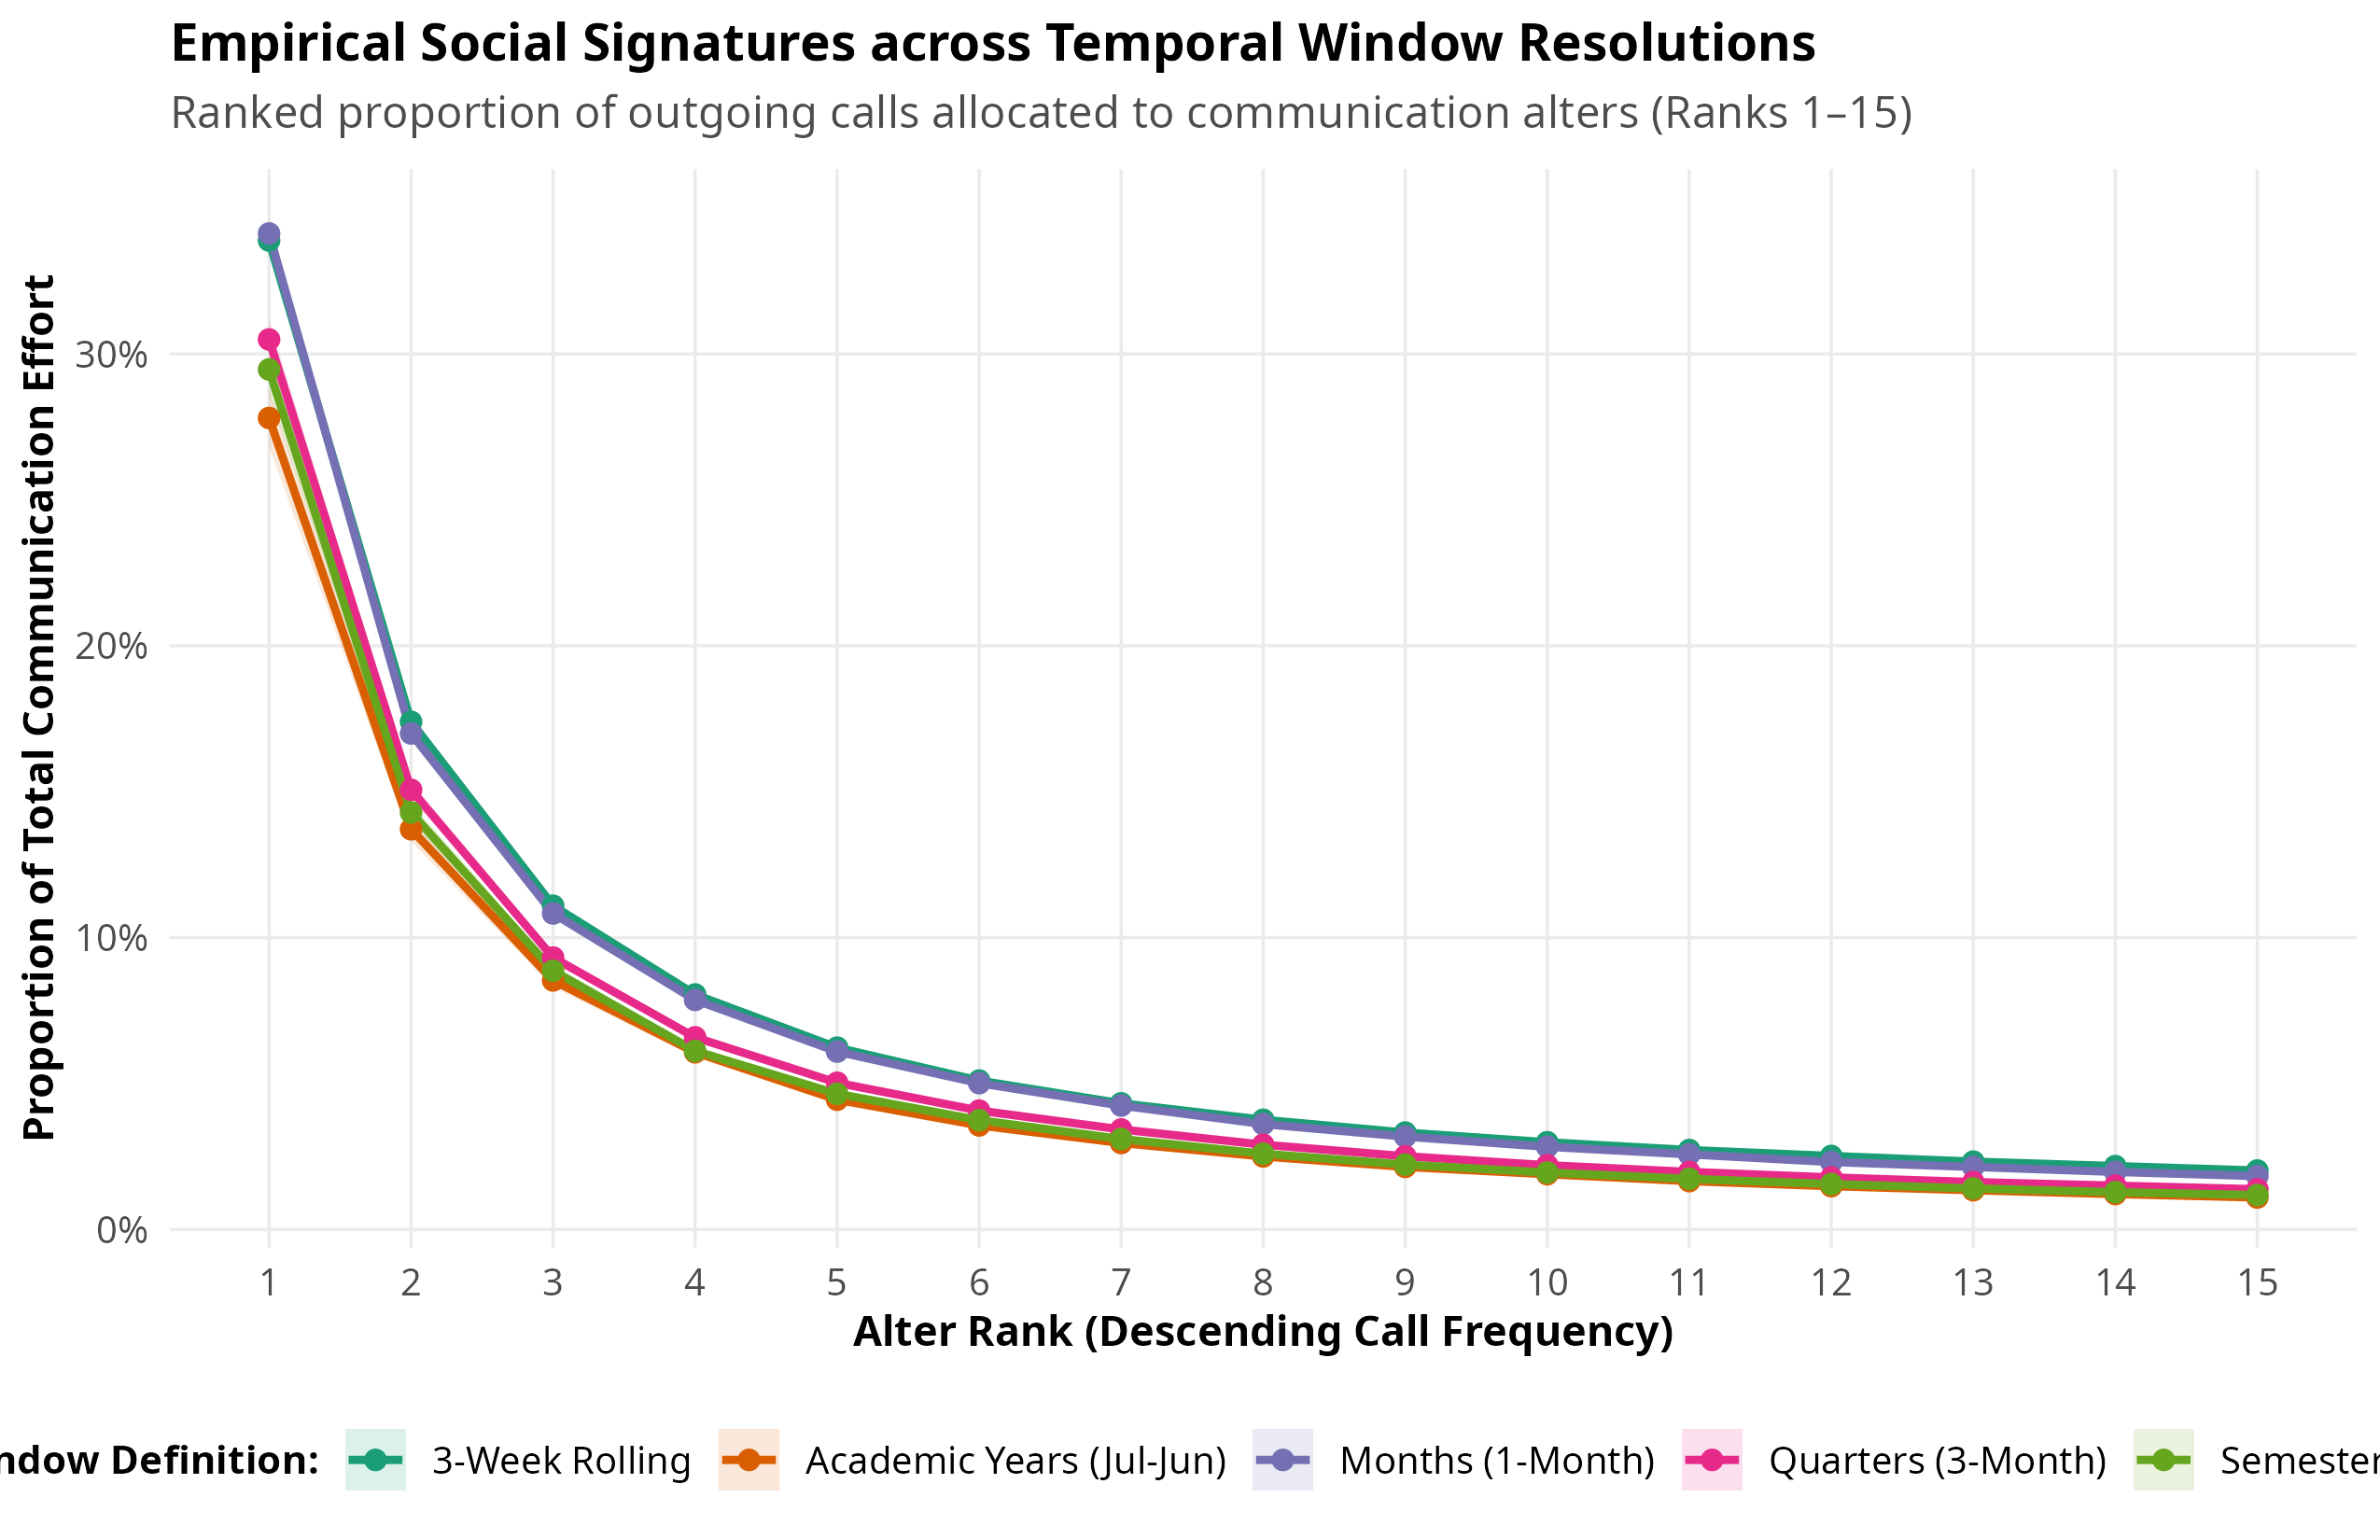
\includegraphics[width=0.9\textwidth]{Plots/fig01_mean_signatures_by_window.png}
\caption{Empirical Social Signatures across Temporal Window Resolutions (Ranks 1--15). Ribbons denote 95\% confidence intervals around the mean interaction proportion.}
\label{fig:mean_signatures}
\end{figure}

\subsection{Robust Intra-Individual Persistence}
Table~\ref{tab:stability_tests} reports the formal statistical comparison between intra-individual self-divergence ($\dself$) and inter-individual reference divergence ($\dref$).

\begin{table}[htbp]
\centering
\caption{Statistical Tests of Social Signature Persistence Across Window Schemes}
\label{tab:stability_tests}
\small
\resizebox{\textwidth}{!}{%
\begin{tabular}{lcccccc}
\toprule
\textbf{Scheme} & \textbf{Egos ($N$)} & \textbf{Mean $\dself$ (SD)} & \textbf{Mean $\dref$ (SD)} & \textbf{Difference} & \textbf{Wilcoxon $V$} & \textbf{$p$-value} \\
\midrule
Academic Years & 388 & 0.0633 (0.0642) & 0.1129 (0.0322) & $-0.0496$ & 6,690.0 & $< 10^{-12}$ \\
Semesters & 290 & 0.0614 (0.0423) & 0.1184 (0.0304) & $-0.0570$ & 1,136.0 & $< 10^{-12}$ \\
Quarters & 227 & 0.0626 (0.0311) & 0.1293 (0.0299) & $-0.0667$ & 50.0 & $< 10^{-12}$ \\
Months & 147 & 0.0877 (0.0305) & 0.1494 (0.0248) & $-0.0617$ & 14.0 & $< 10^{-12}$ \\
Common Cohort (Sem) & 147 & 0.0458 (0.0244) & 0.1057 (0.0250) & $-0.0599$ & 30.0 & $< 10^{-12}$ \\
Common Cohort (Mo) & 147 & 0.0877 (0.0305) & 0.1494 (0.0248) & $-0.0617$ & 14.0 & $< 10^{-12}$ \\
3-Week Rolling & 88 & 0.0495 (0.0147) & 0.1411 (0.0205) & $-0.0916$ & 0.0 & $< 10^{-12}$ \\
2-Week Discrete & 65 & 0.0992 (0.0216) & 0.1439 (0.0167) & $-0.0447$ & 0.0 & $< 10^{-12}$ \\
\bottomrule
\end{tabular}%
}
\end{table}

Across every temporal resolution examined, intra-individual self-divergence is significantly lower than inter-individual reference divergence ($p < 10^{-12}$, Wilcoxon signed-rank test; Cohen's $d > 1.4$). In semester windows, mean self-divergence is 0.0614, compared to a reference divergence of 0.1184 ($V = 1136, p = 1.27 \times 10^{-44}$). Even at fine-grained weekly scales (3-week rolling windows), an individual's signature remains exceptionally consistent across time ($\dself = 0.0495$) relative to the broader population ($\dref = 0.1411, p = 1.90 \times 10^{-16}$). As shown in Figure~\ref{fig:self_vs_ref}, the distributions of self and reference divergence exhibit minimal overlap, confirming that personal communication signatures reflect enduring individual traits.

\begin{figure}[htbp]
\centering
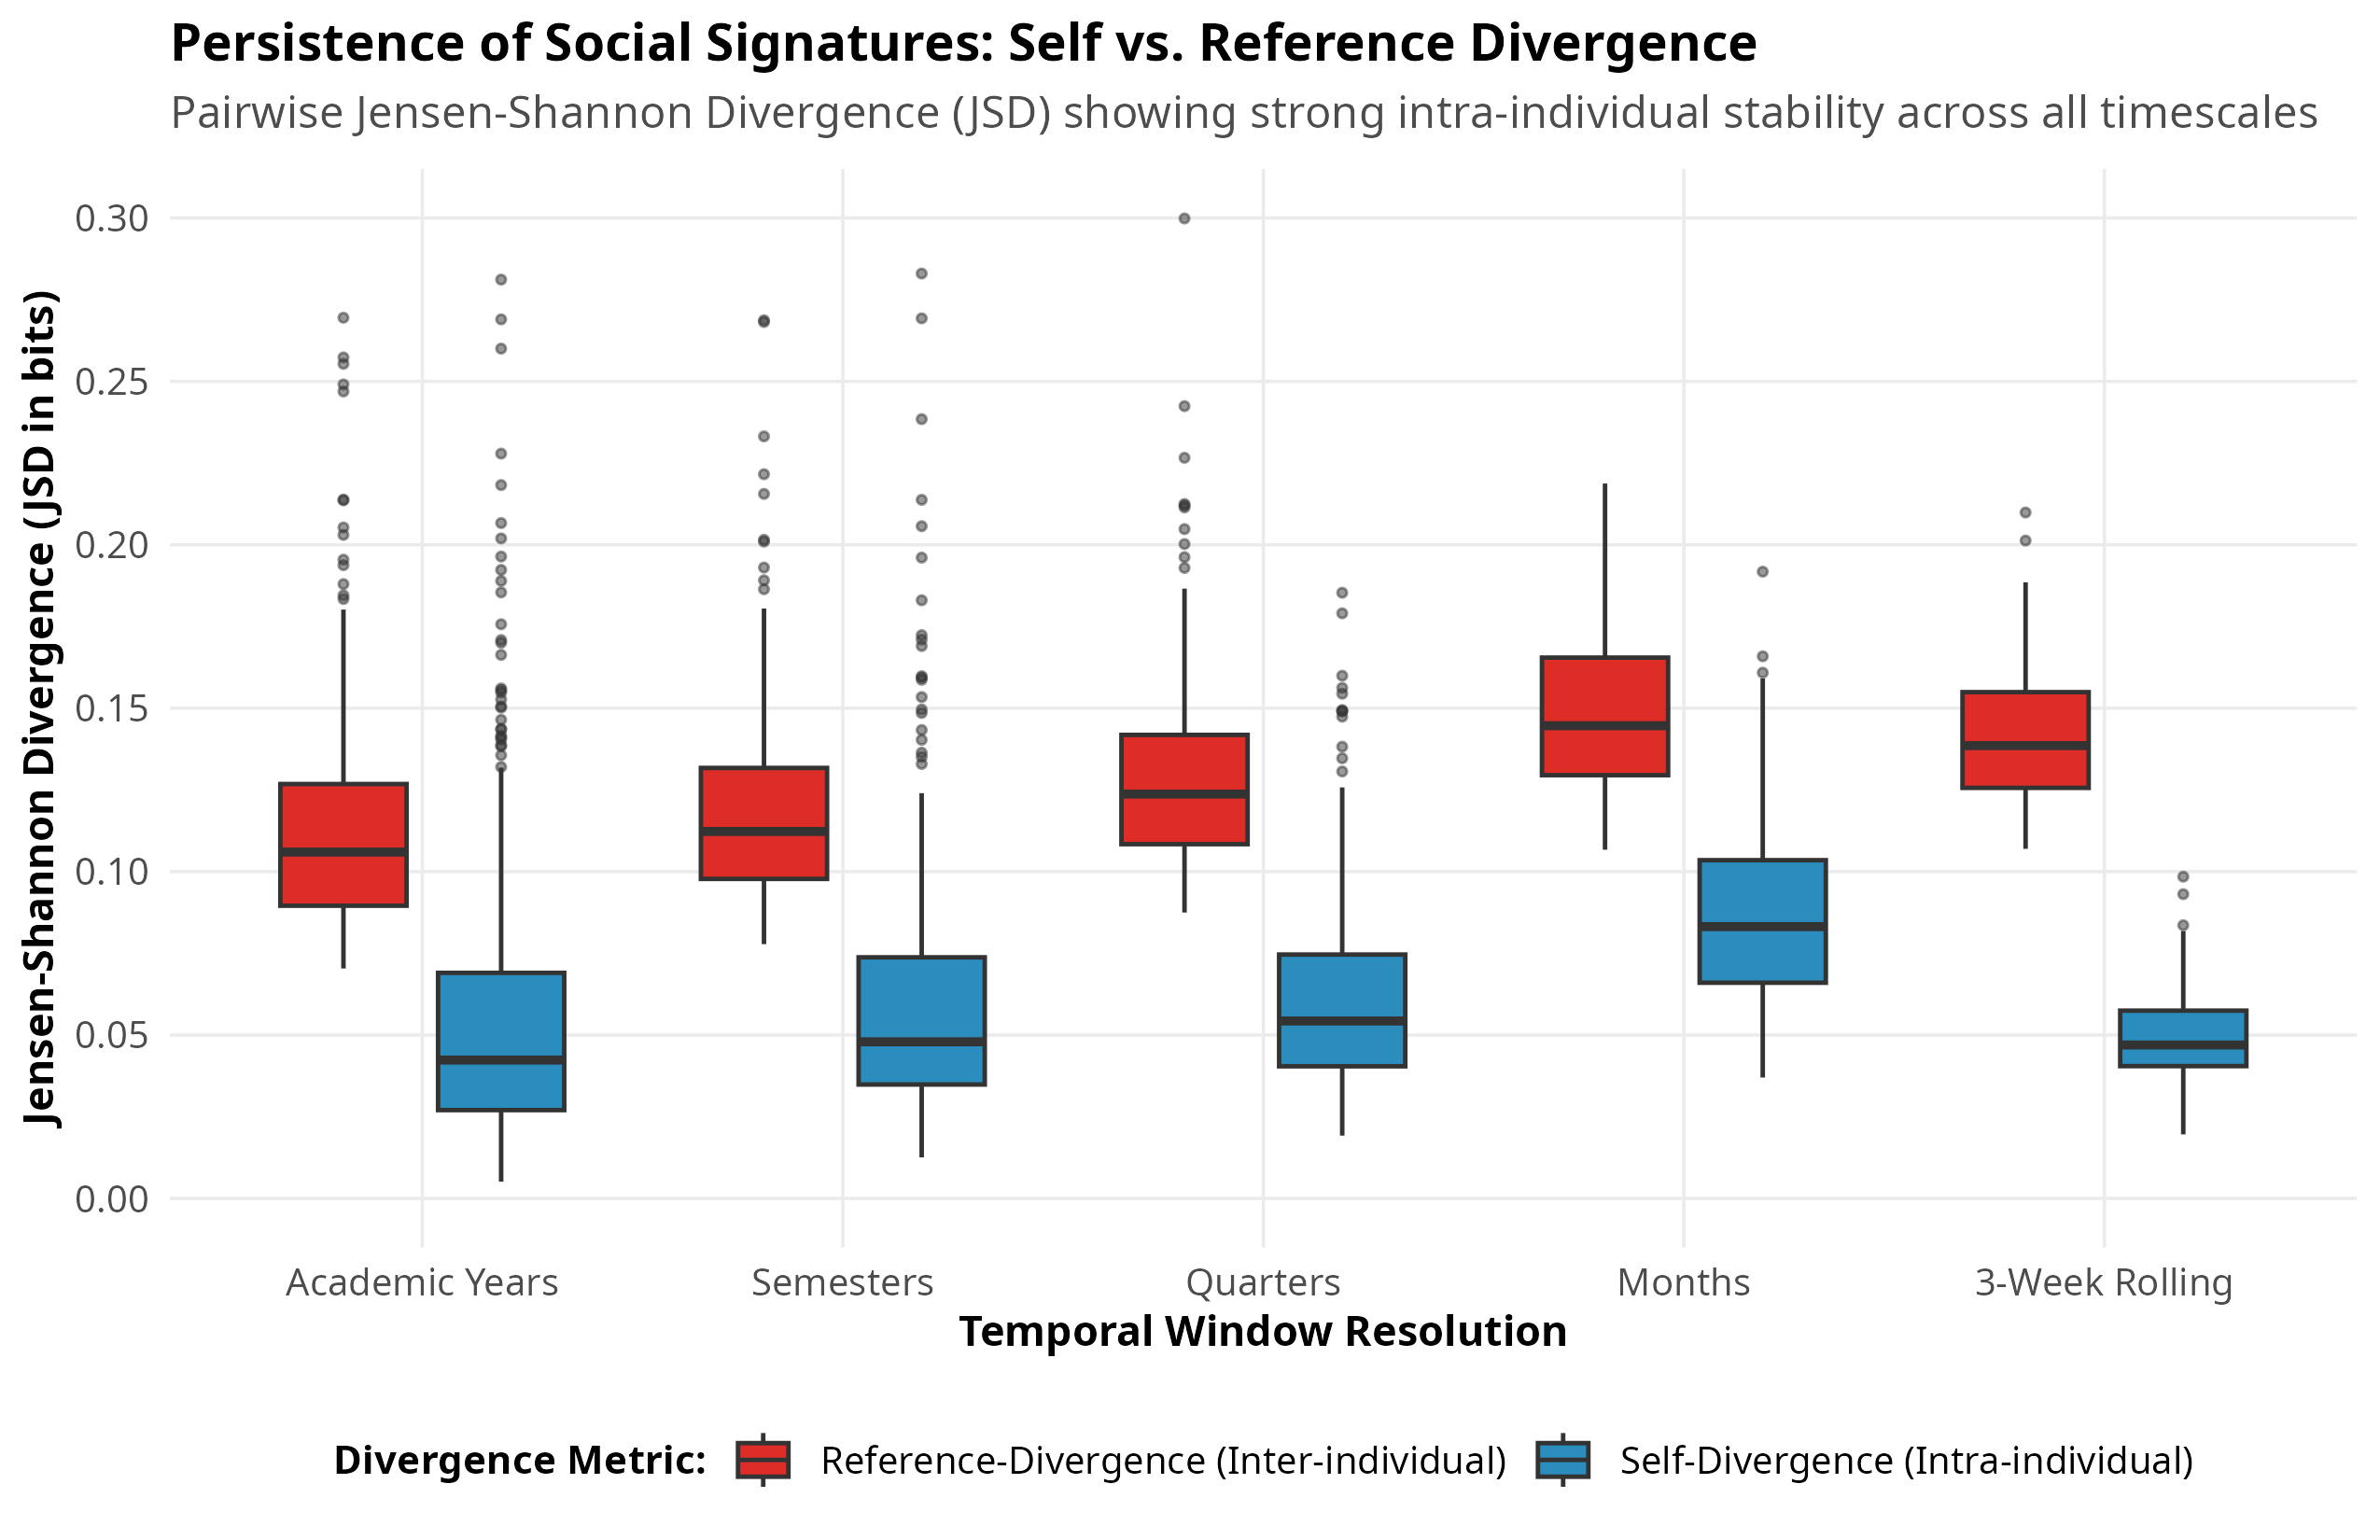
\includegraphics[width=0.9\textwidth]{Plots/fig02_self_vs_ref_divergence.png}
\caption{Persistence of Social Signatures: Self-Divergence vs.\ Reference-Divergence across temporal resolutions. Boxplots show the distribution of individual ego means.}
\label{fig:self_vs_ref}
\end{figure}

\subsection{Parametric Form: Power-Law vs.\ Exponential Decay}
We evaluated two competing functional specifications for the signature curve:
\begin{align}
\text{Power-Law: } p(r) &= c \cdot r^{-\alpha} \iff \log p(r) = \log c - \alpha \log r \\
\text{Exponential: } p(r) &= c \cdot e^{-\beta r} \iff \log p(r) = \log c - \beta r
\end{align}

\begin{table}[htbp]
\centering
\caption{Parametric Model Evaluation Across Window Resolutions}
\label{tab:parametric_models}
\small
\begin{tabular}{lcccccc}
\toprule
\textbf{Scheme} & \textbf{Models ($N$)} & \textbf{Power-Law $\alpha$ (SD)} & \textbf{Power-Law $R^2$} & \textbf{Exp $\beta$} & \textbf{Exp $R^2$} & \textbf{\% PL Preferred} \\
\midrule
Semesters & 1,158 & 1.20 (0.26) & 0.935 & 0.10 & 0.746 & 97.0\% \\
Months & 3,496 & 1.06 (0.37) & 0.883 & 0.23 & 0.771 & 83.8\% \\
\bottomrule
\end{tabular}
\end{table}

As summarized in Table~\ref{tab:parametric_models} and Figure~\ref{fig:power_law_exp}, the power-law model decisively outperforms the exponential specification across both semester and monthly timescales. In semester windows, the power-law specification is preferred by Akaike Information Criterion (AIC) in \textbf{97.0\% of models}, yielding an average $R^2$ of 0.935 (compared to 0.746 for exponential decay). The power-law decay exponent $\alpha$ averages 1.22 ($\text{SD} = 0.25$), reflecting a heavy-tailed allocation profile.

\begin{figure}[htbp]
\centering
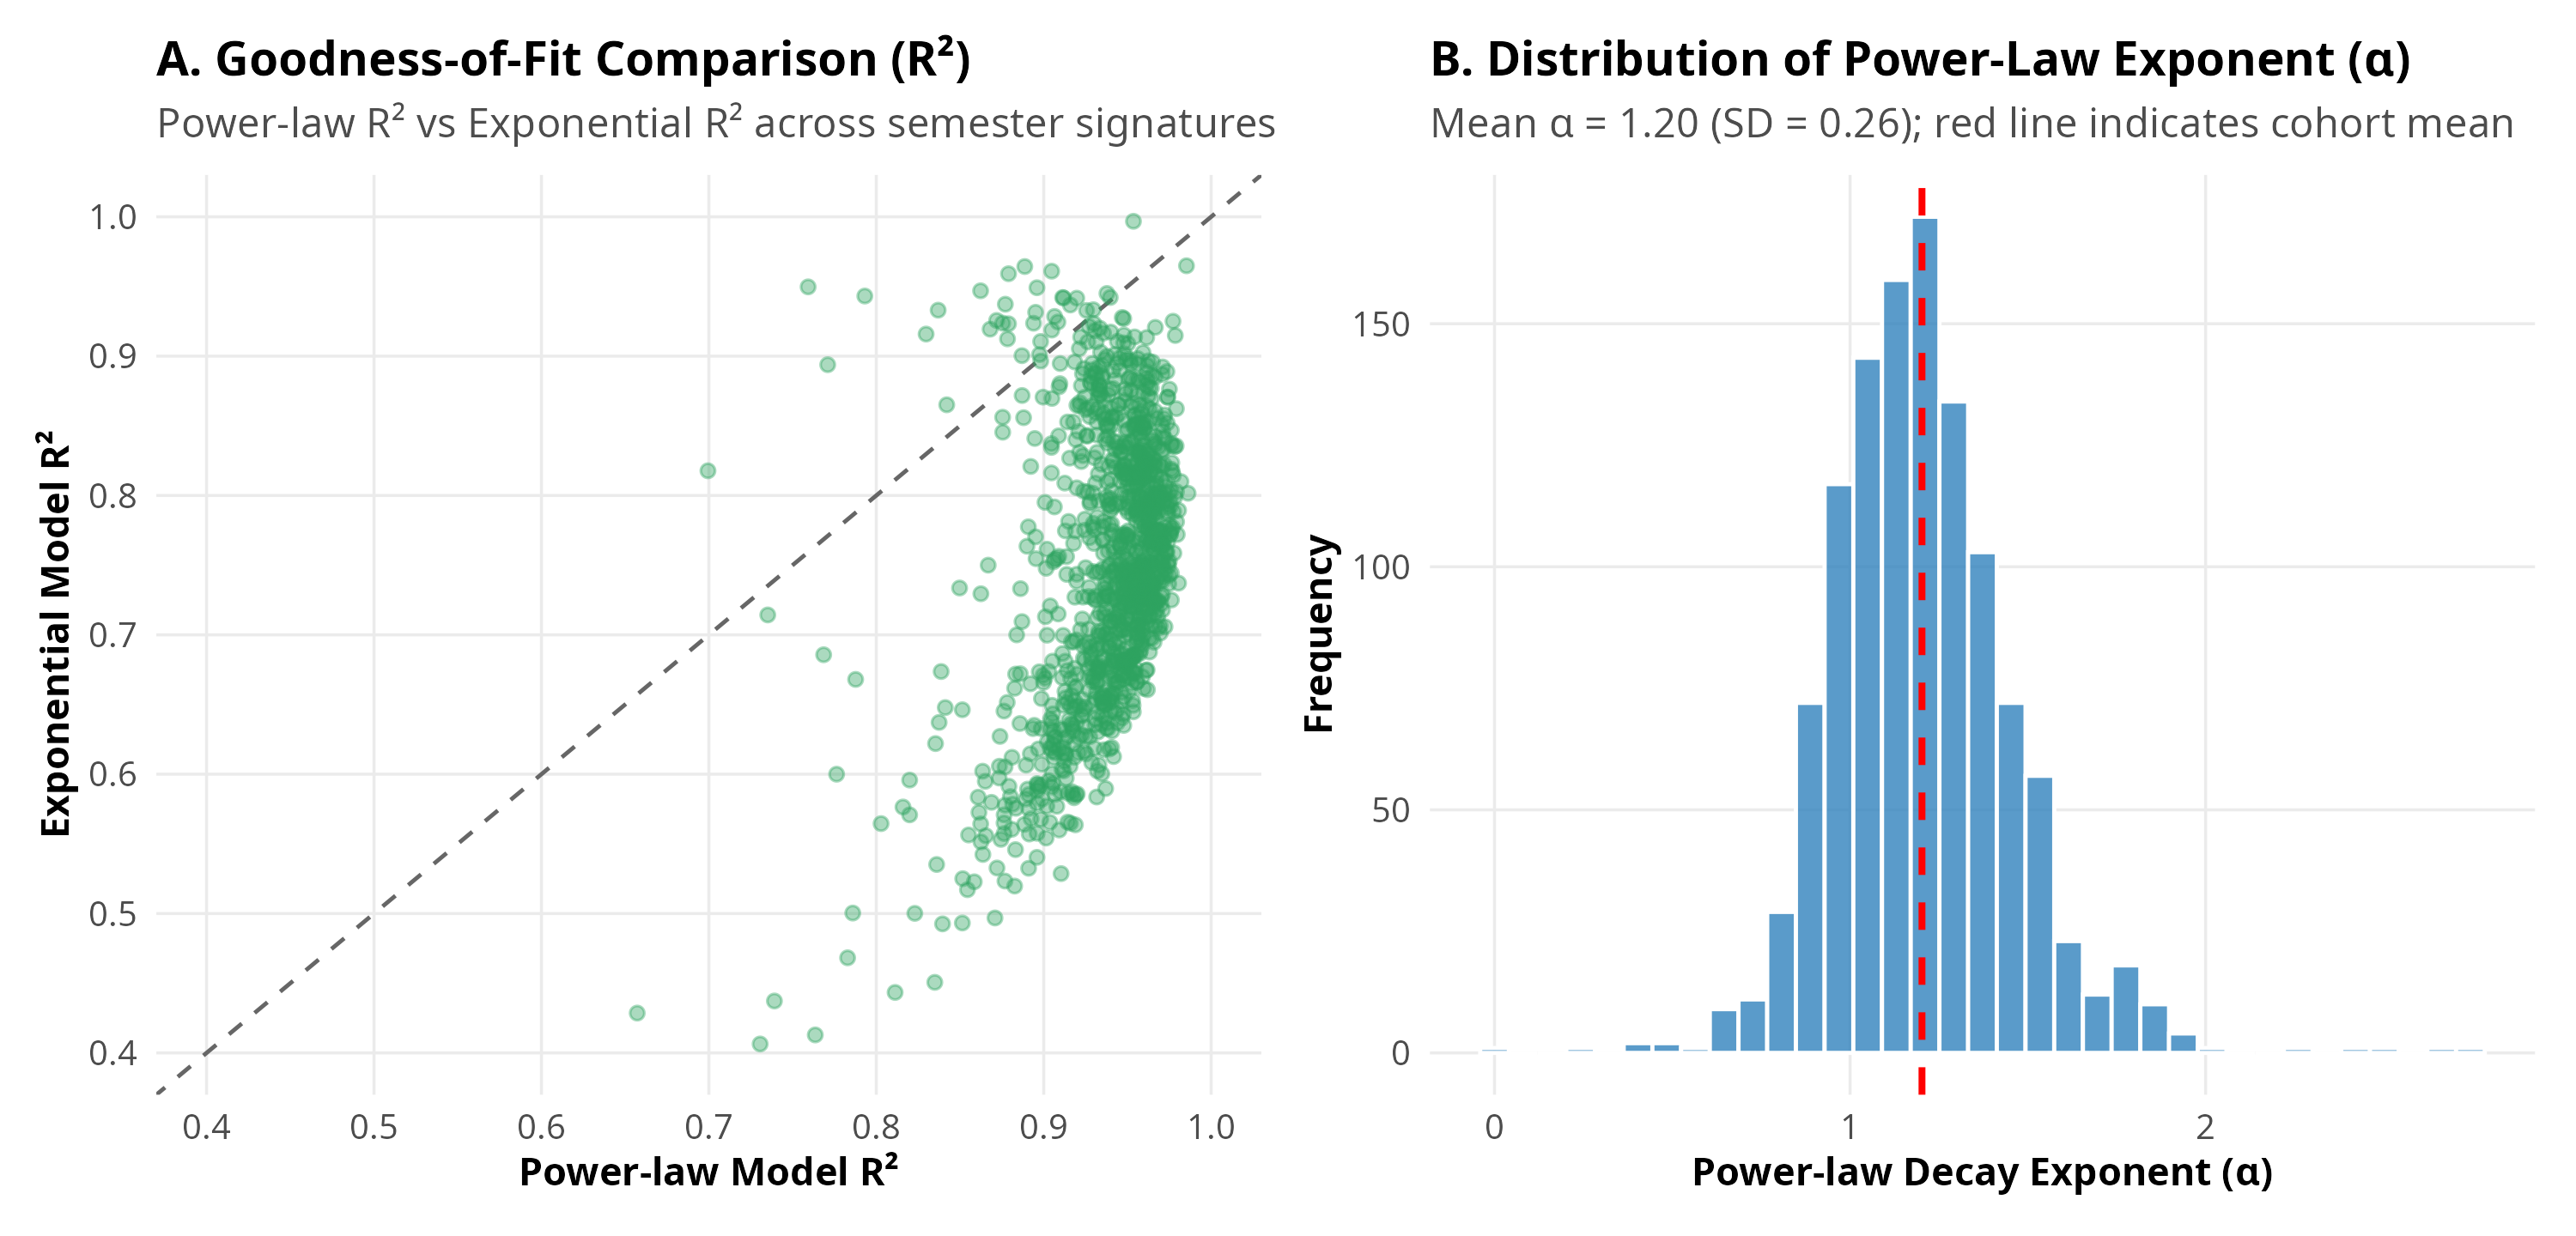
\includegraphics[width=0.95\textwidth]{Plots/fig03_power_law_vs_exponential.png}
\caption{Power-Law vs.\ Exponential Model Fits. (A) Scatterplot of $R^2$ values comparing power-law against exponential fits across semester signatures. (B) Empirical distribution of power-law decay exponent ($\alpha$).}
\label{fig:power_law_exp}
\end{figure}

\subsection{Longitudinal Parameter Convergence and Burn-In}
To establish how long an individual must be observed before their estimated signature parameters stabilize, we tracked the common cohort across cumulative observation lengths from 2 to 24 months (Figure~\ref{fig:burnin}).
\begin{itemize}
    \item At 2 months: Mean $\alpha = 1.16$, with a mean absolute error of 0.188 relative to the 24-month asymptotic value.
    \item At 4 months: Mean absolute error declines to 0.141 ($R^2 = 0.934$).
    \item At 6 to 8 months: Mean absolute error converges below 0.10 ($R^2 = 0.945$).
\end{itemize}

These findings demonstrate that \textbf{6 months of continuous digital observation} provides an optimal burn-in threshold for reliably characterizing personal social signatures in young adult populations.

\begin{figure}[htbp]
\centering
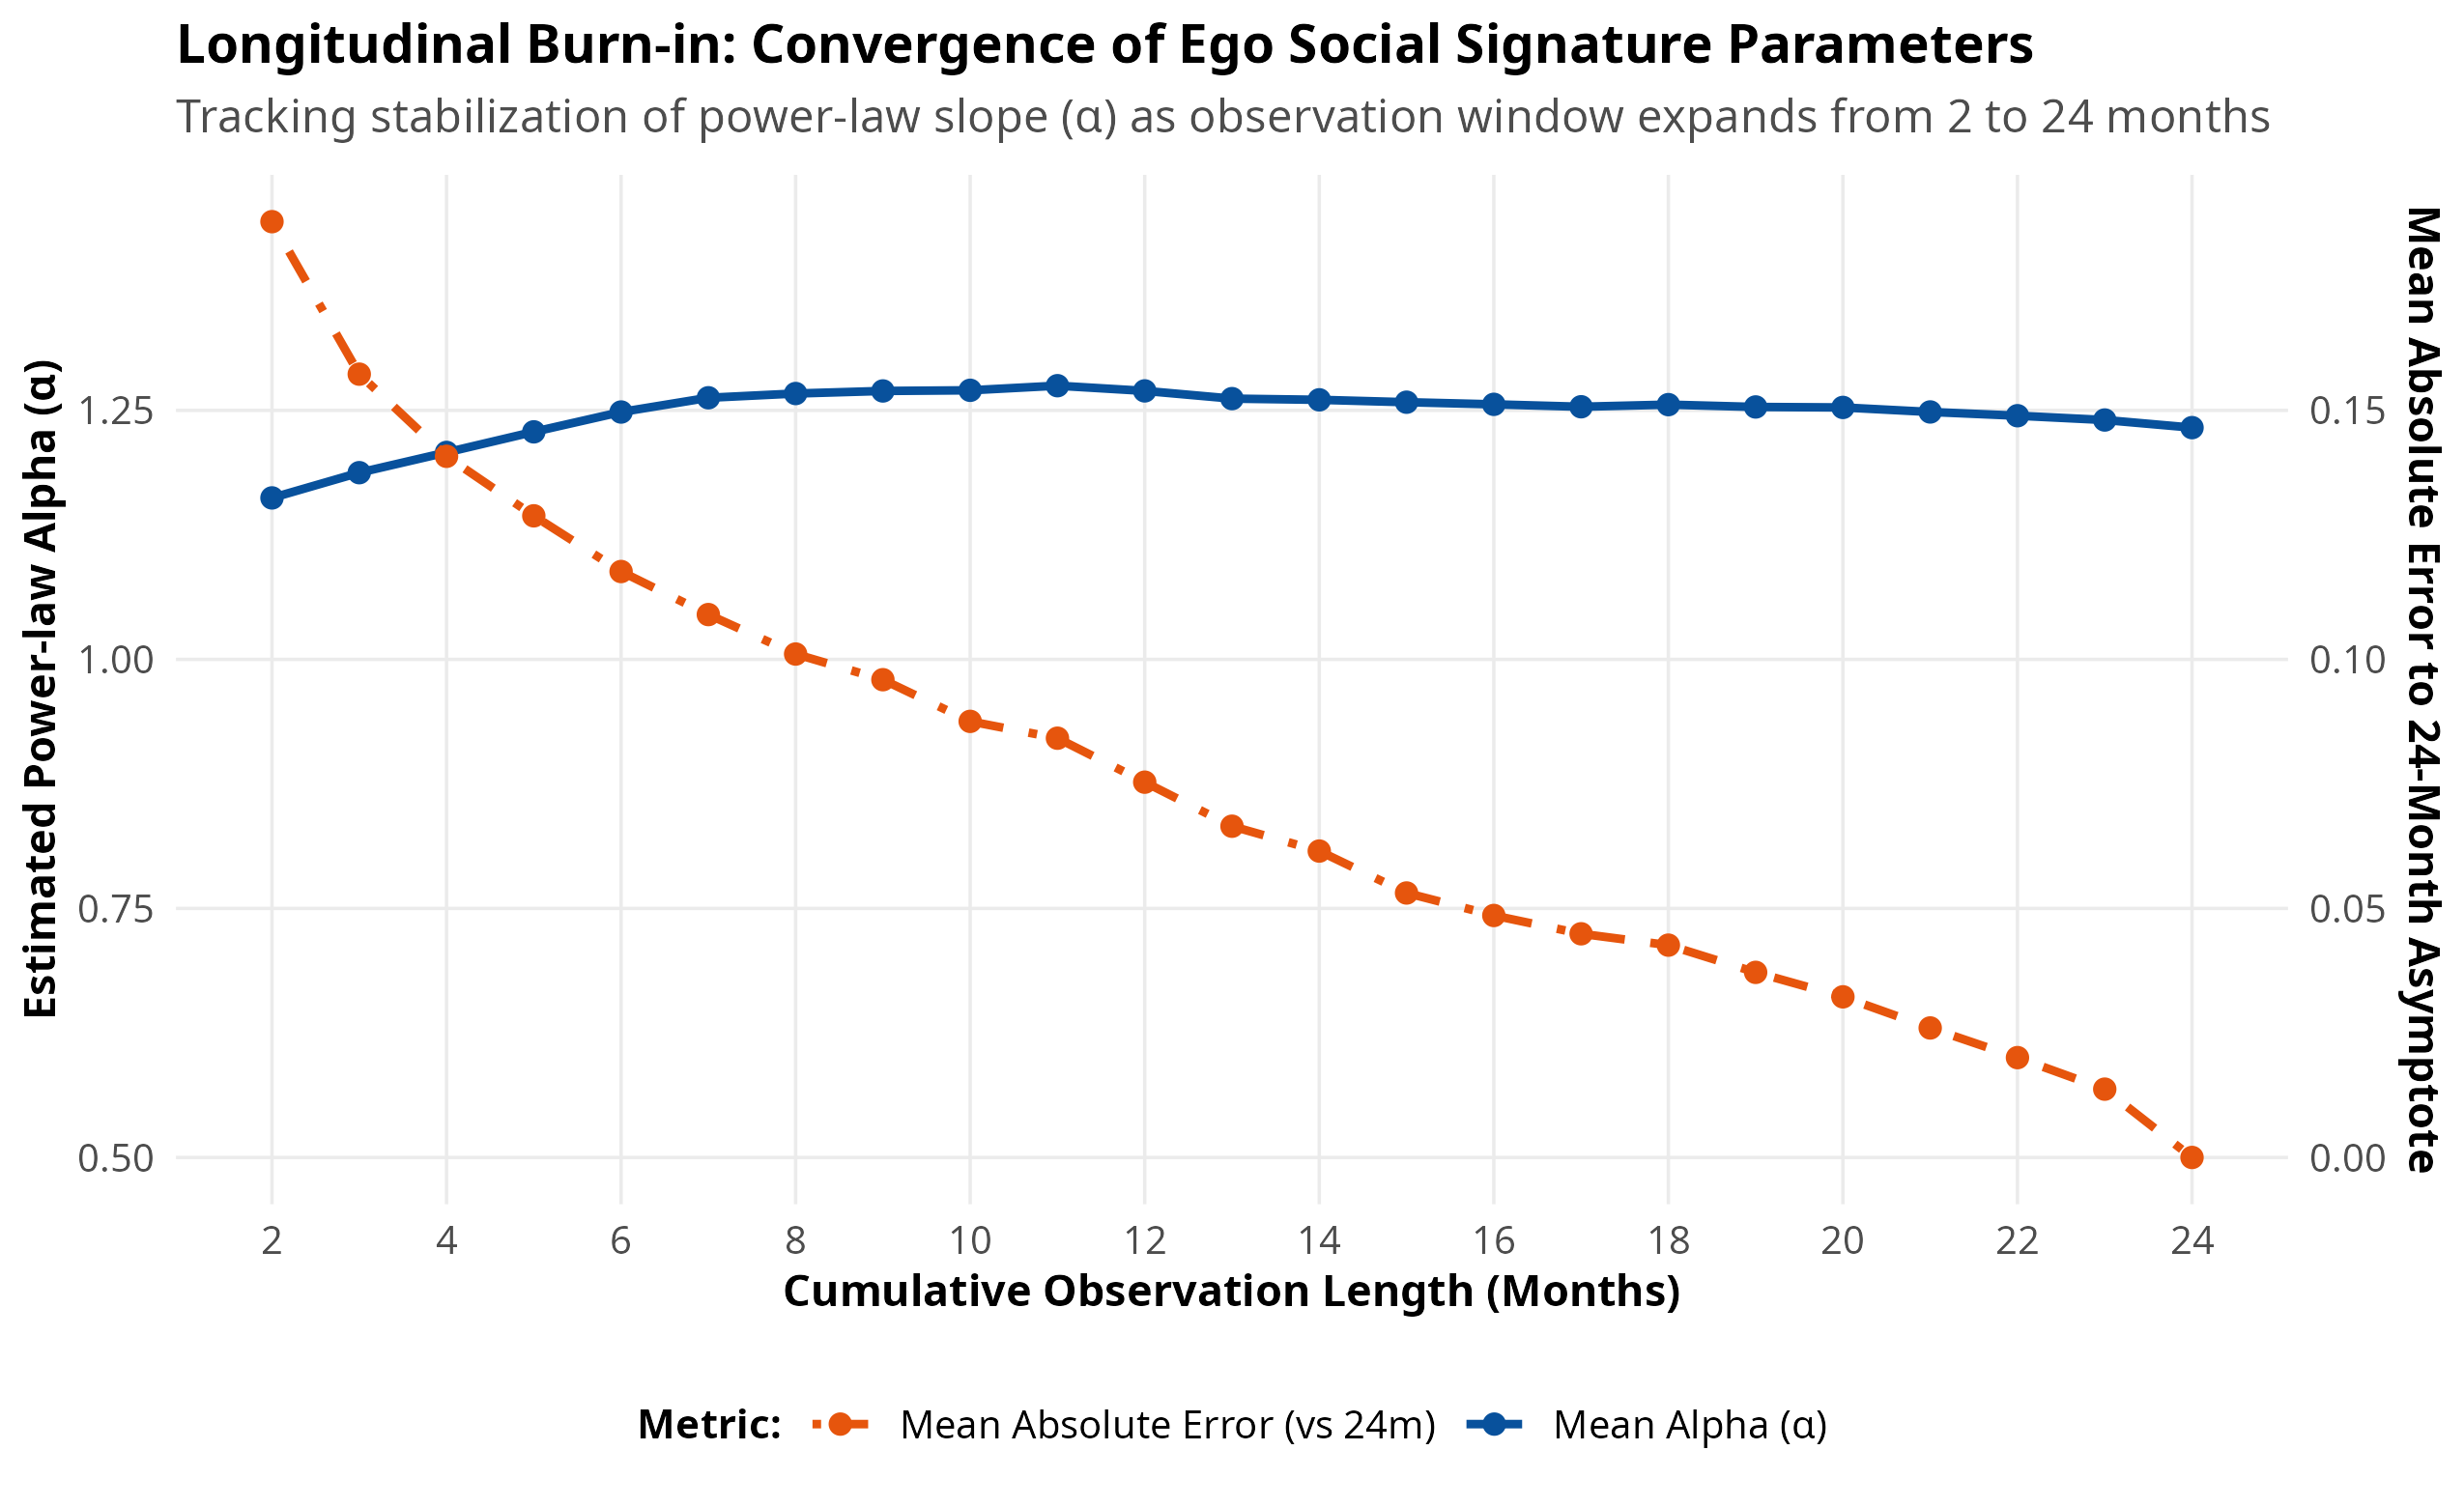
\includegraphics[width=0.9\textwidth]{Plots/fig04_parameter_burnin.png}
\caption{Parameter Burn-In Convergence Over 24 Months. Left axis shows mean estimated power-law $\alpha$; right axis shows mean absolute error relative to the 24-month asymptotic parameter value.}
\label{fig:burnin}
\end{figure}

\section{Theoretical Expansions}

\subsection{Functional Grounding of Communication Ranks in Social Support Dimensions}
While prior literature has treated communication ranks as purely behavioral tallies, we linked $N = 13,174$ call-ranked dyads to longitudinal network surveys recording relationship categories and support functions across six theoretical Dunbar tiers (Table~\ref{tab:support_tiers} and Figure~\ref{fig:support_tiers}).

\begin{table}[htbp]
\centering
\caption{Relational Composition and Support Functions Across Signature Rank Tiers ($N = 13,174$ Dyads)}
\label{tab:support_tiers}
\small
\resizebox{\textwidth}{!}{%
\begin{tabular}{lccccccc}
\toprule
\textbf{Rank Tier} & \textbf{Ties ($N$)} & \textbf{\% Family} & \textbf{\% Friend} & \textbf{\% Emotional} & \textbf{\% Advice} & \textbf{\% Companionship} & \textbf{\% Financial} \\
\midrule
Rank 1 (Core) & 950 & 69.7\% & 16.9\% & 85.4\% & 87.6\% & 80.6\% & 64.1\% \\
Ranks 2--3 & 1,713 & 62.2\% & 34.0\% & 77.1\% & 80.1\% & 79.8\% & 45.1\% \\
Ranks 4--5 & 1,426 & 41.4\% & 56.9\% & 70.0\% & 73.0\% & 81.9\% & 24.2\% \\
Ranks 6--10 & 2,743 & 24.2\% & 74.4\% & 60.7\% & 64.3\% & 78.2\% & 12.4\% \\
Ranks 11--20 & 3,011 & 14.3\% & 84.5\% & 48.1\% & 53.6\% & 74.4\% & 7.1\% \\
Ranks $>20$ & 3,331 & 9.2\% & 87.8\% & 39.1\% & 44.0\% & 69.5\% & 4.4\% \\
\bottomrule
\end{tabular}%
}
\end{table}

The findings illuminate the qualitative architecture underlying social signatures:
\begin{enumerate}
    \item \textbf{The Kinship Core}: Rank 1 is heavily dominated by family members (69.7\% kin, primarily parents and romantic partners), who provide the structural foundation of instrumental, advice, and financial support (64.1\% financial assistance, 87.6\% advice, 85.4\% emotional support).
    \item \textbf{The Friendship Transition}: A sharp structural crossover occurs between Ranks 3 and 5. At Ranks 2--3, family members still constitute 62.2\% of ties; by Ranks 4--5, peer friends constitute the majority (56.9\%), rising to 87.8\% beyond Rank 20.
    \item \textbf{Differentiated Support Gradient}: Emotional support (85.4\% at Rank 1) and advice support (87.6\% at Rank 1) fall monotonically across tiers (dropping to 39.1\% and 44.0\% for outer ties). In sharp contrast, companionship remains elevated across all tiers (80.6\% at Rank 1, 81.9\% at Ranks 4--5, and 69.5\% beyond Rank 20), demonstrating that peripheral communication ties serve primary social leisure and recreational functions.
\end{enumerate}

\begin{figure}[htbp]
\centering
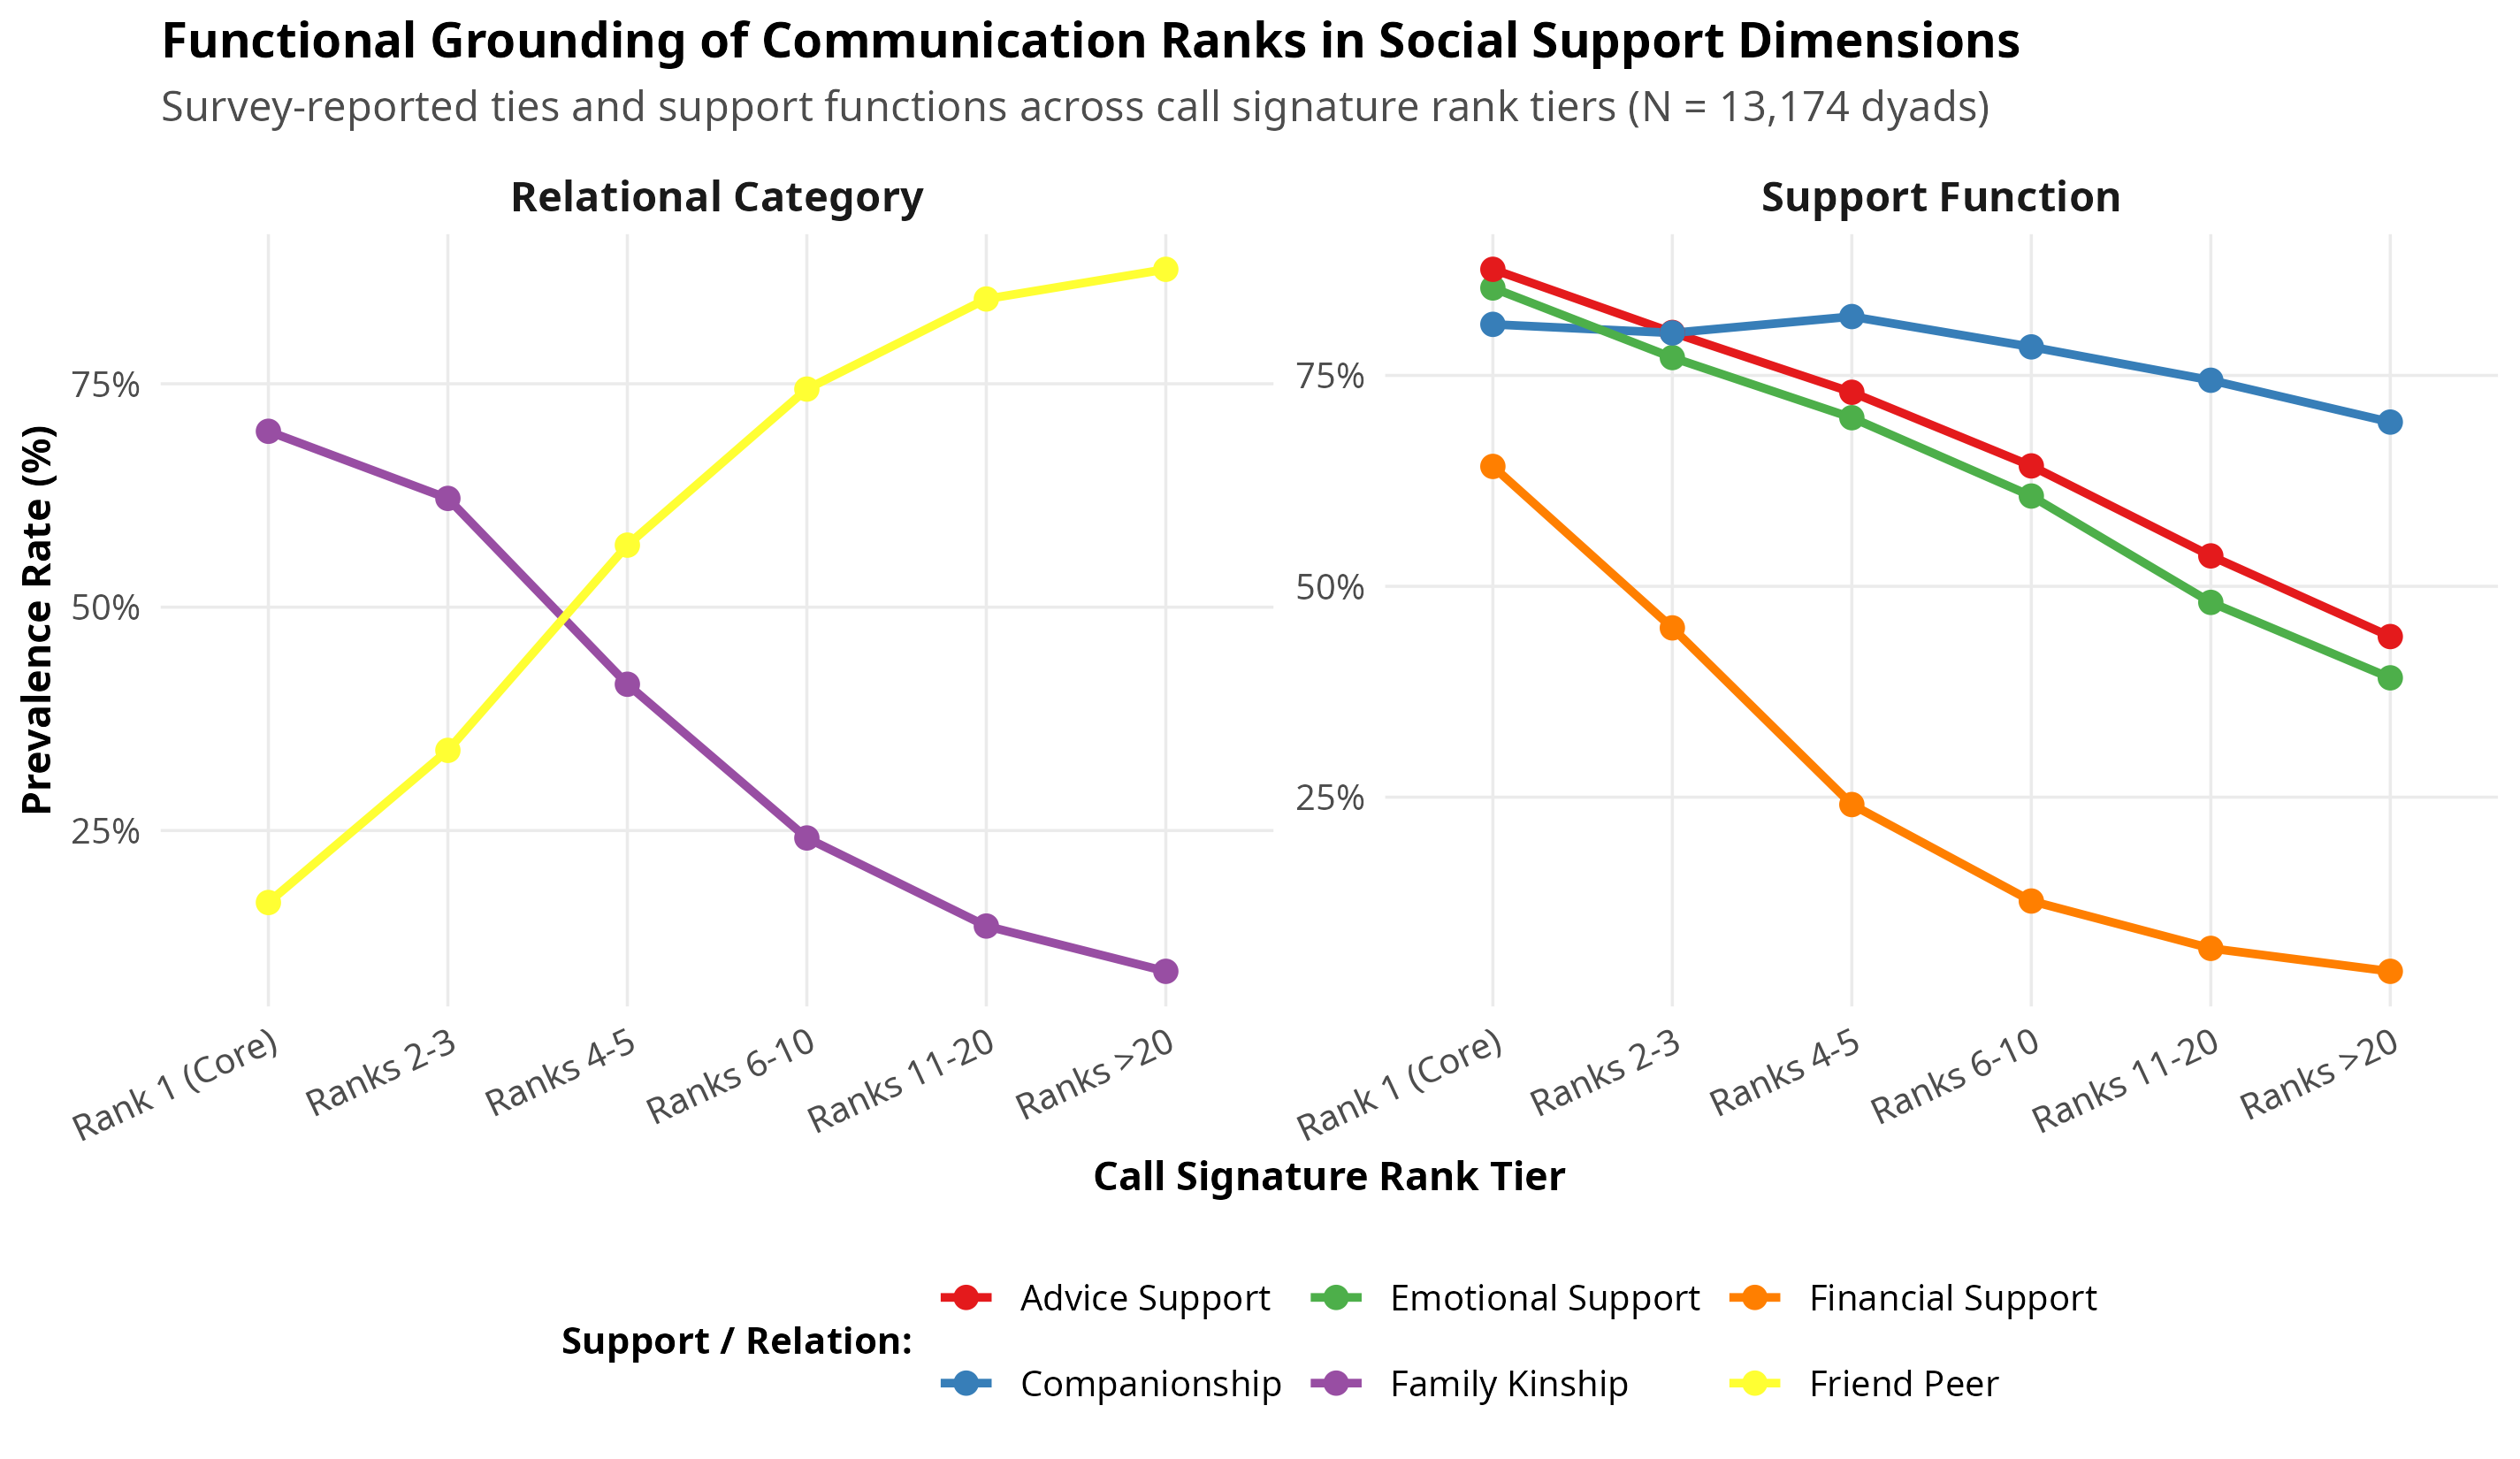
\includegraphics[width=0.95\textwidth]{Plots/fig05_rank_by_support_tiers.png}
\caption{Functional Support Dimensions Across Signature Rank Tiers. Shows prevalence rates of relational categories (left panel) and substantive support provisions (right panel).}
\label{fig:support_tiers}
\end{figure}

\subsection{The ``Slot-Filling'' Dynamic: Alter Turnover vs.\ Signature Stability}
A central theoretical puzzle in network science is how an ego's signature can remain stable despite frequent alter replacement. We calculated the dyadic Jaccard turnover between consecutive semesters:
\begin{equation}
\Turnover_{i,w} = 1 - \frac{|A_{i,w} \cap A_{i,w+1}|}{|A_{i,w} \cup A_{i,w+1}|}
\end{equation}
where $A_{i,w}$ denotes the set of active alters for ego $i$ in window $w$.

Remarkably, \textbf{alter turnover between consecutive semesters averages 80.1\% ($\text{SD} = 0.076$)}. Despite replacing four out of five alters every six months, egos maintain an average self-divergence of only 0.0614. In 59.1\% of consecutive semester intervals, the single top-ranked alter was retained; even when the top alter was replaced, the overall self-divergence increased only modestly (from 0.0431 to 0.0785, Figure~\ref{fig:turnover}). 

This pattern provides direct empirical confirmation of the \textbf{slot-filling hypothesis}: an individual maintains a predefined cognitive template for relationship allocation, seamlessly slotting new social entrants into vacant relational positions without perturbing their structural allocation curve.

\begin{figure}[htbp]
\centering
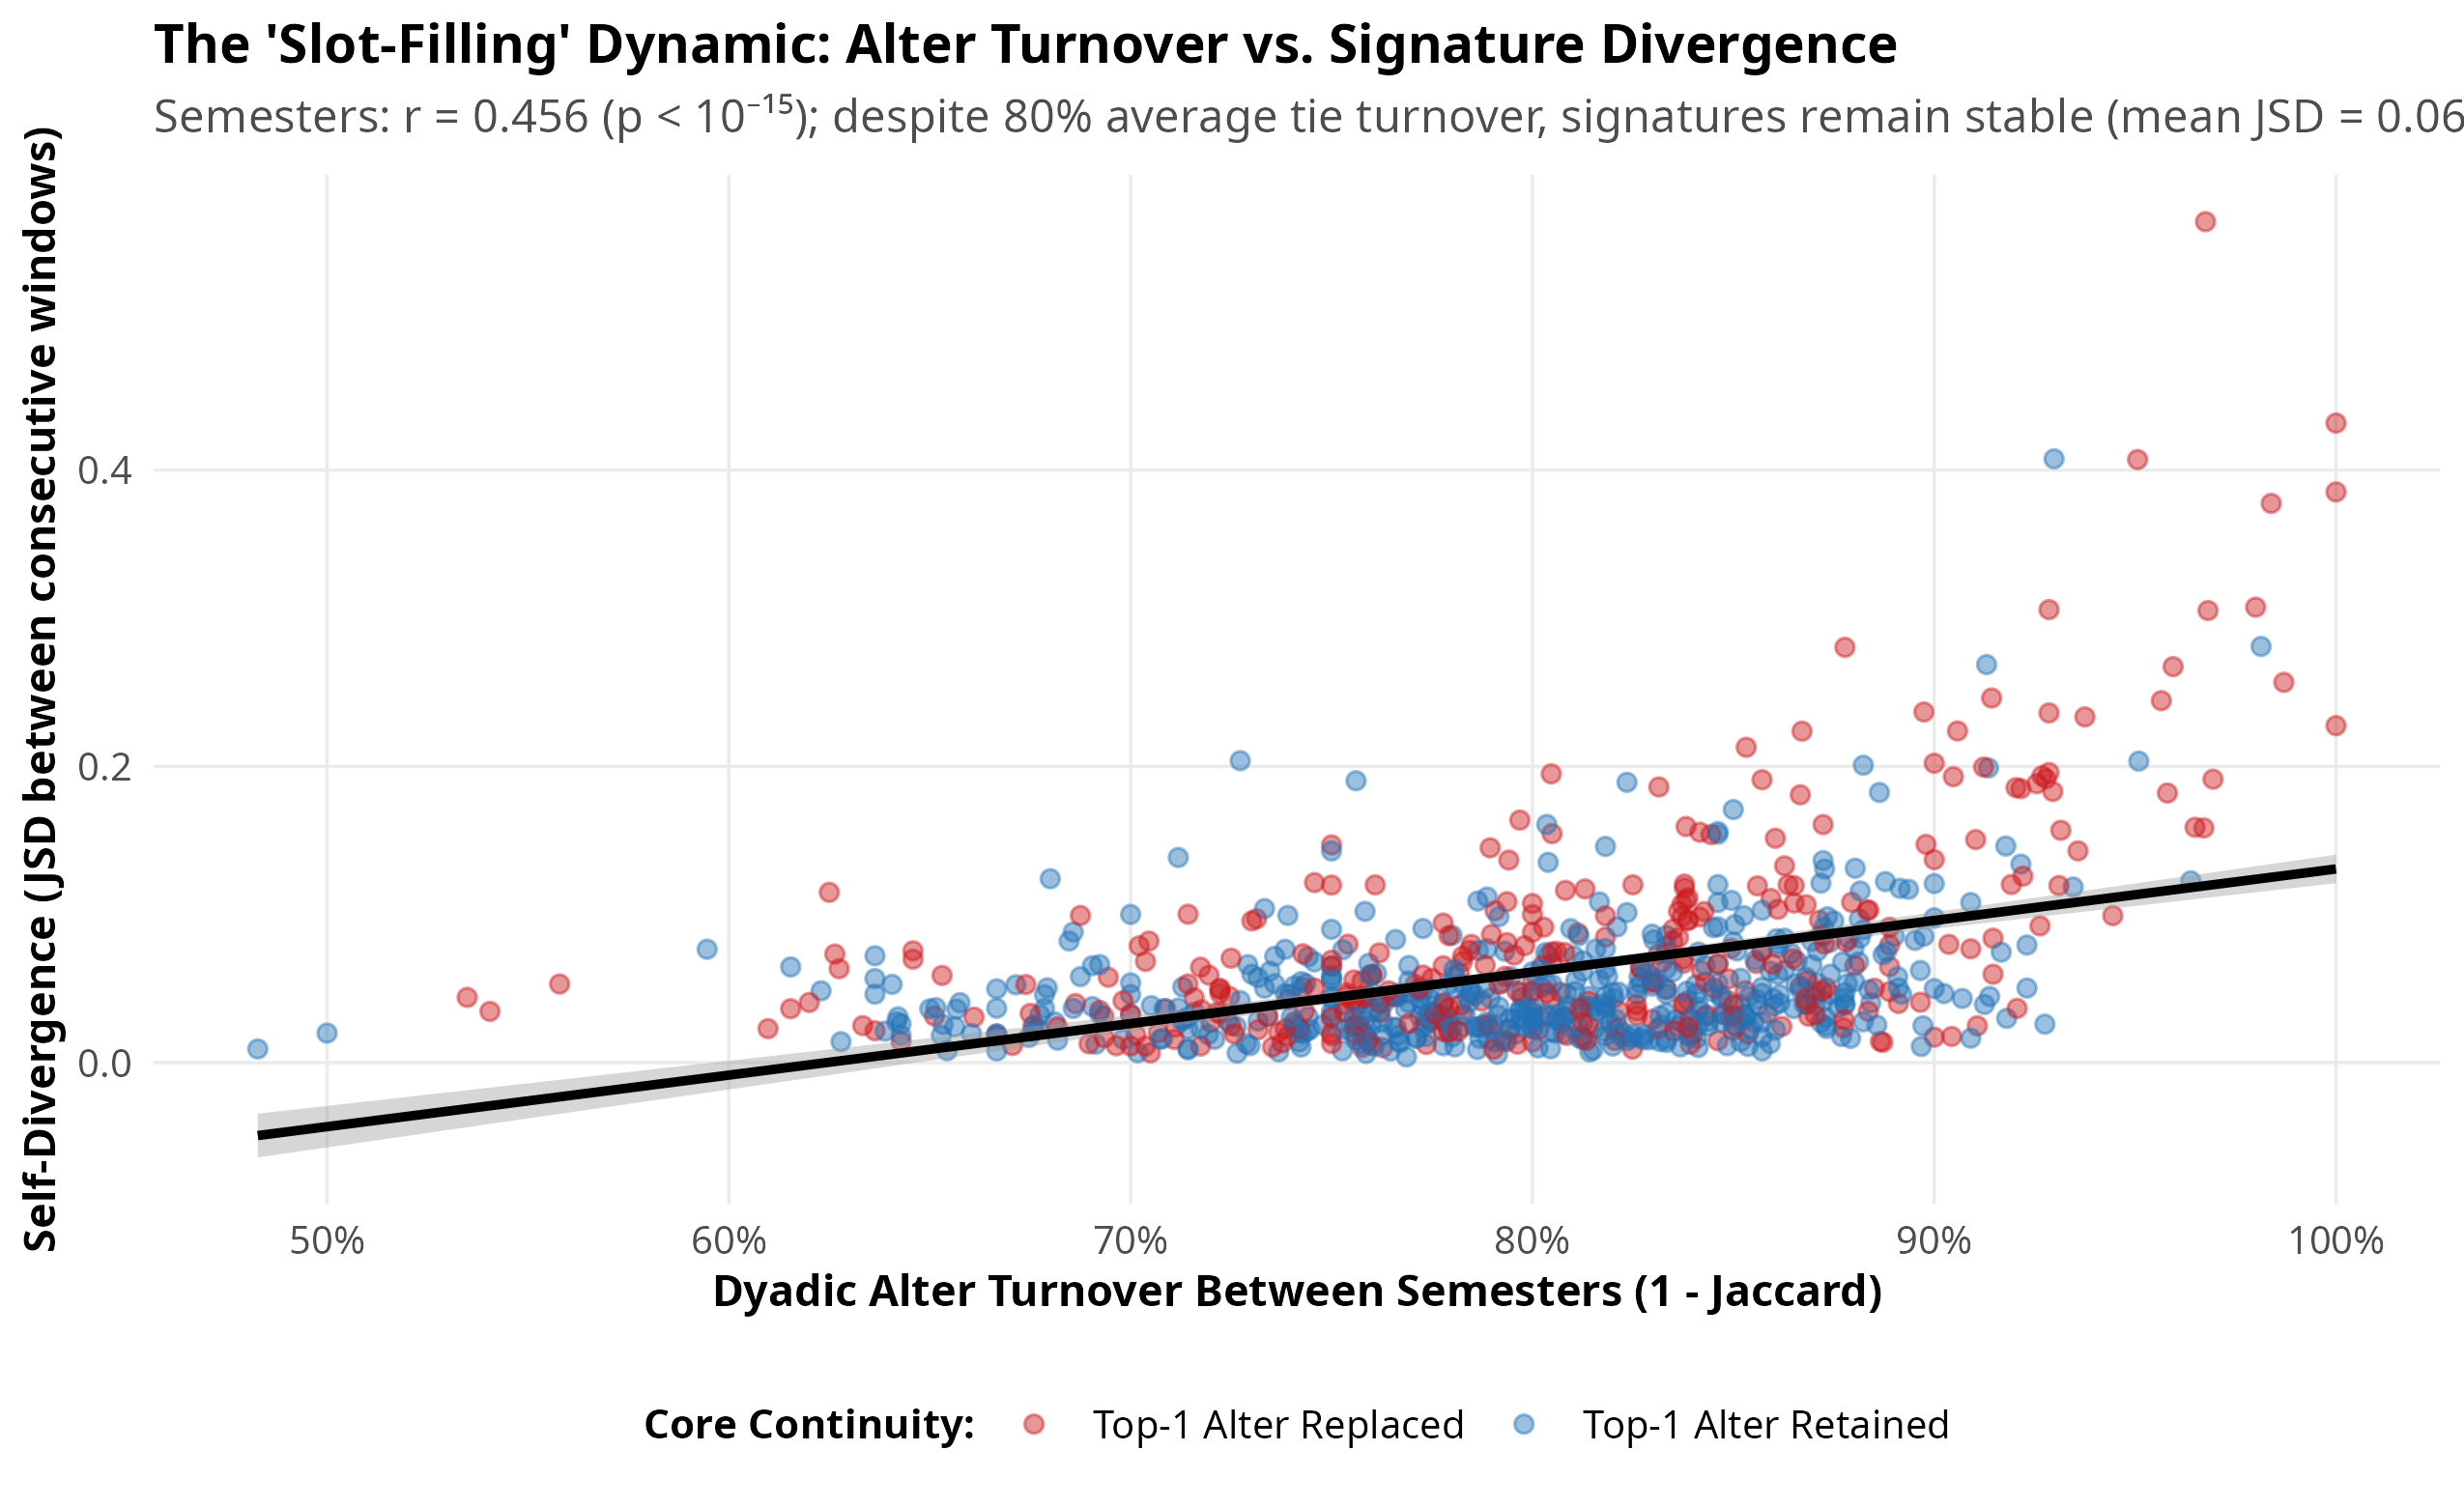
\includegraphics[width=0.9\textwidth]{Plots/fig06_turnover_vs_stability.png}
\caption{The `Slot-Filling' Dynamic: Alter Turnover vs.\ Signature Divergence ($r = 0.456, p < 10^{-15}$). Blue points denote intervals where the Rank 1 alter was retained; red points denote intervals where the Rank 1 alter was replaced.}
\label{fig:turnover}
\end{figure}

\subsection{Multilevel Panel Models of Signature Divergence}
To identify the structural and psychological drivers of signature mutation over time, we estimated linear mixed-effects panel models with ego random intercepts:
\begin{equation}
\JSD_{it} = \beta_0 + \beta_1 \Turnover_{it} + \beta_2 \Delta \mathrm{Activity}_{it} + \mathbf{X}_{it}\boldsymbol{\gamma} + u_i + \epsilon_{it}
\end{equation}
where $u_i \sim \mathcal{N}(0, \sigma_u^2)$ and $\epsilon_{it} \sim \mathcal{N}(0, \sigma_\epsilon^2)$.

\begin{table}[htbp]
\centering
\caption{Multilevel Linear Mixed-Effects Models Predicting Signature Self-Divergence ($\JSD$)}
\label{tab:multilevel_models}
\small
\resizebox{\textwidth}{!}{%
\begin{tabular}{lccc}
\toprule
\textbf{Predictor Term} & \textbf{Model 1 (Turnover)} & \textbf{Model 2 (Topology)} & \textbf{Model 3 (Integrated)} \\
\midrule
Intercept & $-0.237^{***}\ (0.0195)$ & $-0.200^{***}\ (0.0224)$ & $-0.171^{***}\ (0.0320)$ \\
Alter Turnover ($1 - \Jaccard$) & $0.373^{***}\ (0.0242)$ & $0.336^{***}\ (0.0240)$ & $0.351^{***}\ (0.0287)$ \\
\% Activity Change ($|\Delta\mathrm{Calls}|/\mathrm{Calls}$) & -- & $0.0014^{***}\ (0.0002)$ & $0.0014^{***}\ (0.0002)$ \\
Egonet Clustering Coefficient & -- & $-0.0145\ (0.0157)$ & $-0.0066\ (0.0153)$ \\
Egonet Density & -- & $0.0029\ (0.0154)$ & -- \\
Baseline Extraversion & -- & -- & $-0.0069^\dagger\ (0.0038)$ \\
Baseline Neuroticism & -- & -- & $-0.0090^\dagger\ (0.0049)$ \\
Baseline CES-D Depression & -- & -- & $0.0002\ (0.0005)$ \\
\midrule
Observations & 870 & 870 & 870 \\
Ego Groups & 290 & 290 & 290 \\
\bottomrule
\multicolumn{4}{l}{\footnotesize Standard errors in parentheses. $^{***}p < 0.001$, $^{**}p < 0.01$, $^*p < 0.05$, $^\dagger p < 0.10$.}
\end{tabular}%
}
\end{table}

As reported in Table~\ref{tab:multilevel_models}, alter turnover is the primary driver of signature divergence ($\beta = 0.351, p < 10^{-15}$), followed by large shifts in communication volume ($\beta = 0.0014, p < 10^{-10}$). Net of turnover, egonet clustering does not significantly alter signature stability, underscoring that signatures reflect cognitive rather than purely topological constraints.

\subsection{Personality Determinants of Signature Steepness}
What psychological dispositions generate steep (core-concentrated) versus flat (diffuse) social signatures? Regressing ego-mean power-law decay exponents ($\alpha_i$) on Big Five personality traits and personal network degree (Table~\ref{tab:personality_models} and Figure~\ref{fig:personality}) reveals:

\begin{table}[htbp]
\centering
\caption{Personality Determinants of Social Signature Power-Law Alpha ($\alpha_i$)}
\label{tab:personality_models}
\small
\begin{tabular}{lcccc}
\toprule
\textbf{Term} & \textbf{Estimate} & \textbf{Std.\ Error} & \textbf{$t$ value} & \textbf{$p$-value} \\
\midrule
(Intercept) & $0.680^{***}$ & 0.162 & 4.21 & $< 0.001$ \\
Extraversion & $-0.017$ & 0.017 & $-1.01$ & 0.314 \\
Neuroticism & $0.098^{***}$ & 0.019 & 5.08 & $< 0.001$ \\
Agreeableness & $0.063^{*}$ & 0.025 & 2.49 & 0.014 \\
Conscientiousness & 0.021 & 0.023 & 0.89 & 0.374 \\
Openness & 0.014 & 0.027 & 0.53 & 0.598 \\
Personal Network Degree & $-0.004^\dagger$ & 0.002 & $-1.76$ & 0.080 \\
\midrule
\multicolumn{5}{l}{\footnotesize $N = 290$ egos, $R^2 = 0.124, F(6, 283) = 6.69, p < 0.000001$.}
\end{tabular}
\end{table}

\textbf{Neuroticism is a highly significant, positive predictor of signature steepness ($\beta = 0.098, t = 5.08, p < 10^{-6}$)}. Individuals high in neuroticism exhibit hyper-concentrated communication profiles, funneling the vast majority of their interactions into one or two primary alters while under-investing in intermediate and outer bands. Agreeableness also exhibits a modest positive association with concentration ($\beta = 0.063, p = 0.014$). In contrast, extraversion tends to flatten signatures toward broader alter engagement.

\begin{figure}[htbp]
\centering
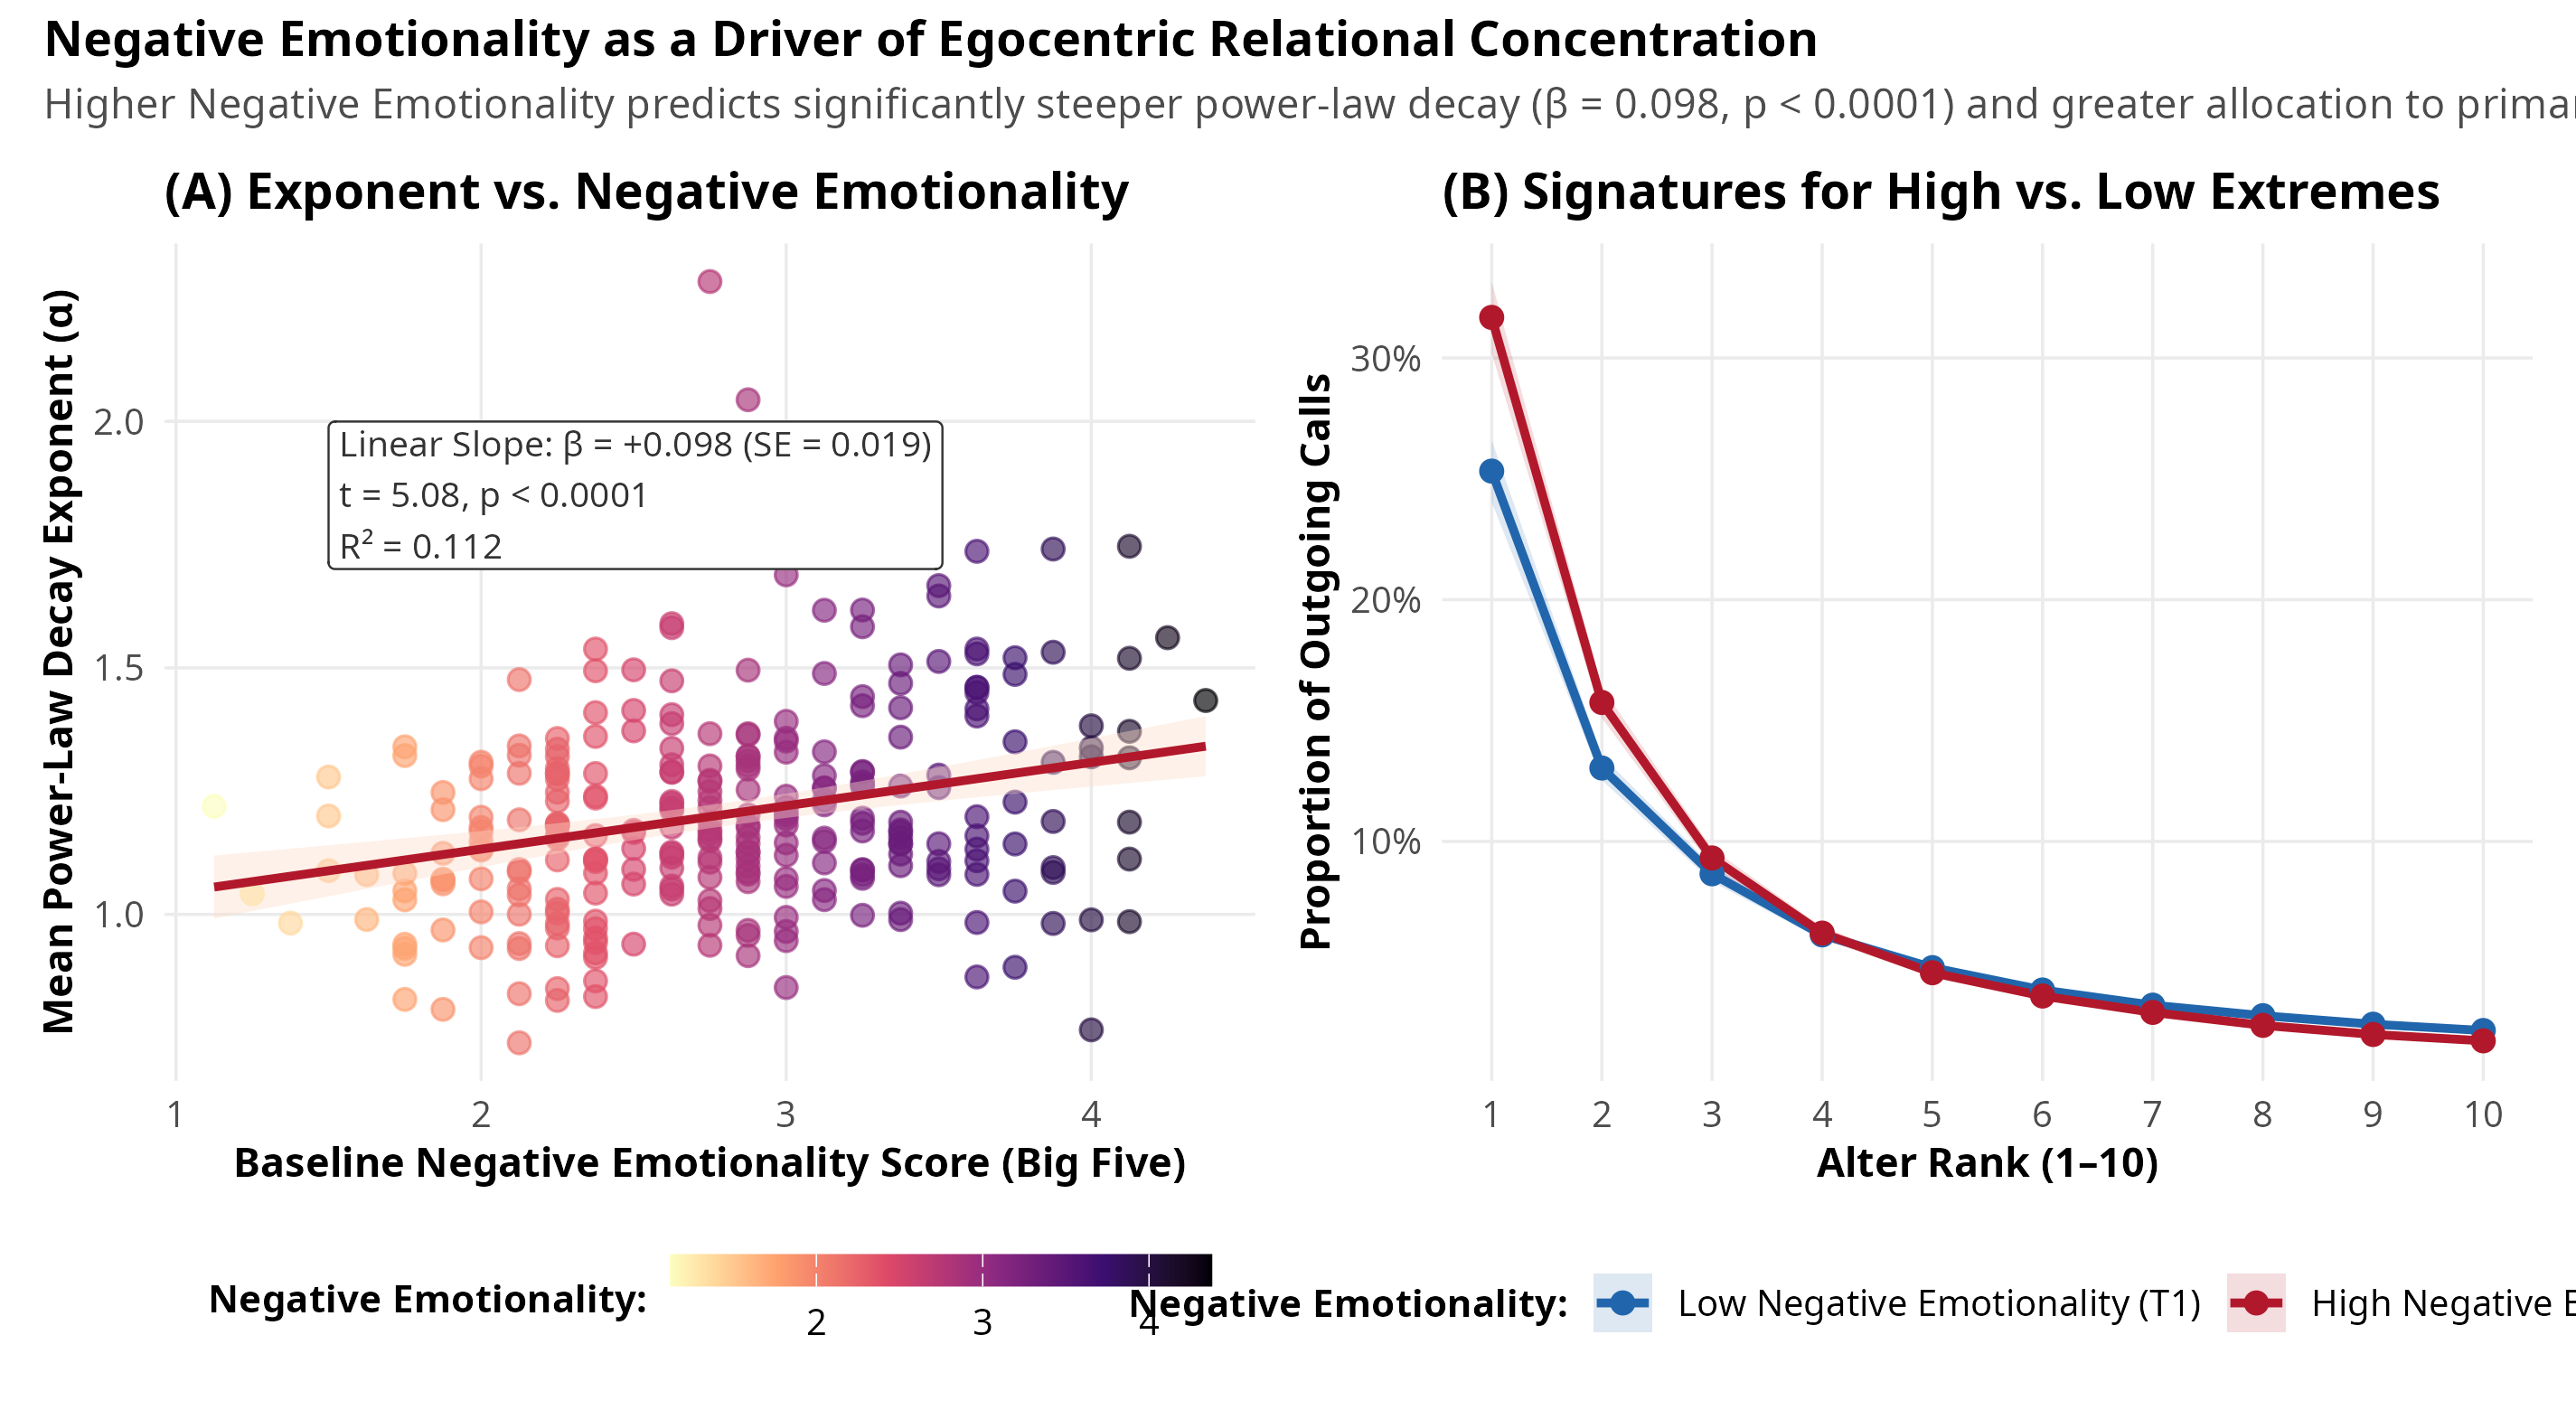
\includegraphics[width=0.9\textwidth]{Plots/fig07_personality_signature_effects.png}
\caption{Personality Predictors of Social Signature Alpha. Neuroticism score predicts significantly steeper power-law decay ($\beta = 0.098, p < 10^{-6}$). Points colored by individual Extraversion score.}
\label{fig:personality}
\end{figure}

\section{Discussion and Conclusion}

By linking continuous passive smartphone logs with multi-wave sociocentric surveys and psychological batteries in the NetHealth cohort, this study provides definitive empirical backing for social signature theory while advancing the paradigm into sociological and psychological domains.

Our key findings are threefold:
\begin{enumerate}
    \item \textbf{Unambiguous Persistence}: Social signatures in NetHealth are robustly persistent across timescales ranging from 3-week rolling windows to multi-year academic terms. An individual's signature divergence across time is less than half the divergence observed between random peers.
    \item \textbf{Substantive Grounding}: Social signature ranks are not arbitrary artifacts of call logging; they map directly to evolutionary Dunbar tiers. Rank 1 represents a specialized kin-based support hub, Ranks 2--5 represent the core emotional confidant circle, and ranks beyond 5 represent peer-based companionship.
    \item \textbf{The Psychological Signature}: The shape of the social signature is anchored in personality. Neuroticism drives individuals to adopt steep, risk-averse, hyper-concentrated allocation strategies, while agreeable and emotionally stable individuals allocate attention across broader social circles.
\end{enumerate}

Future research should leverage high-resolution wearable sensing (Fitbit physical activity, sleep regularity, and colocation traces) to examine whether disruptions in social signature equilibrium serve as early-warning biomarkers for loneliness, academic distress, and depressive episodes during major life transitions.

\bibliographystyle{plainnat}
\bibliography{references}

\end{document}
